% ============================================================================
% Template Jurnal Penulisan Ilmiah - Teknik Informatika
% Universitas Gunadarma
% ============================================================================
\documentclass[12pt,a4paper,twocolumn]{article}

% --- Packages ---------------------------------------------------------------
\usepackage[T1]{fontenc}
\usepackage[utf8]{inputenc}
\usepackage[indonesian]{babel}       % Bahasa Indonesia support
\usepackage{mathptmx}                % Times New Roman font
\usepackage{geometry}                % Page margins
\usepackage{setspace}                % Line spacing
\usepackage{graphicx}                % Images
\usepackage{amsmath,amssymb}         % Mathematical equations
\usepackage{caption}                 % Caption formatting
\usepackage{natbib}                  % Author-date citation style
\usepackage{url}                     % URL formatting
\usepackage{booktabs}                % Professional tables
\usepackage{array}                   % Extended table columns
\usepackage{titlesec}                % Section title formatting
\usepackage{fancyhdr}                % Headers and footers
\usepackage{abstract}                % Abstract formatting
\usepackage{indentfirst}             % Indent first paragraph of sections
\usepackage{listings}                % Code listings
\usepackage{xcolor}                  % Color support for listings
\usepackage{tabularx}                % Flexible-width tables
\usepackage{multirow}                % Multi-row cells in tables
\usepackage{float}                   % Force float placement with [H]
\usepackage{hyperref}                % Hyperlinks (load last)

% --- Listings Setup ---------------------------------------------------------
\lstset{
    basicstyle       = \ttfamily\scriptsize,
    keywordstyle     = \color{blue}\bfseries,
    commentstyle     = \color{gray},
    stringstyle      = \color{red},
    breaklines       = true,
    frame            = single,
    numbers          = none,
    showstringspaces = false,
    tabsize          = 2,
    captionpos       = b
}

% --- Page Layout ------------------------------------------------------------
\geometry{
    a4paper,
    left   = 3cm,
    right  = 3cm,
    top    = 3cm,
    bottom = 3cm
}

% --- Spacing ----------------------------------------------------------------
\onehalfspacing                      % 1.5 line spacing
\setlength{\columnsep}{1cm}          % Column separation

% --- Section Formatting -----------------------------------------------------
% Sections: uppercase, bold, centered, 12pt
\titleformat{\section}
    {\normalfont\normalsize\bfseries\MakeUppercase}
    {}
    {0pt}
    {}
\titlespacing*{\section}{0pt}{12pt}{6pt}

% Subsections: bold, left-aligned, 12pt (no numbering as per format)
\titleformat{\subsection}
    {\normalfont\normalsize\bfseries}
    {}
    {0pt}
    {}
\titlespacing*{\subsection}{0pt}{10pt}{4pt}

% Remove section numbering
\setcounter{secnumdepth}{0}

% --- Caption Formatting -----------------------------------------------------
% Table captions: above table, centered, title case
% Figure captions: below figure, centered, title case
\captionsetup{
    font       = {small},            % 10pt caption text
    labelfont  = {bf},               % Bold "Tabel 1." / "Gambar 1."
    labelsep   = period,             % Period after number
    justification = centering,
    singlelinecheck = false
}
\captionsetup[table]{position = above}
\captionsetup[figure]{position = below}

% --- Citation Style ---------------------------------------------------------
\bibliographystyle{apalike}          % Author-date style (Kotler, 2000)

% --- Hyperlink Setup --------------------------------------------------------
\hypersetup{
    colorlinks  = true,
    linkcolor   = black,
    citecolor   = black,
    urlcolor    = blue
}

% ============================================================================
% DOCUMENT START
% ============================================================================
\begin{document}

% --- Title ------------------------------------------------------------------
% Title is written in the full page width (single column)
\twocolumn[
\begin{@twocolumnfalse}
\begin{center}

% JUDUL
{\bfseries PENGEMBANGAN MARKETPLACE E-COMMERCE TERINTEGRASI \\
DENGAN FITUR MULTI-SELLER DAN MULTI-ORDER}

\vspace{12pt}

% AUTHORS
{\normalsize
Muhammad Hisyam\textsuperscript{1} Atit Pertiwi\textsuperscript{2}
}

\vspace{8pt}

% AFFILIATIONS
{\small
\textsuperscript{1}Fakultas Teknologi Industri, Universitas Gunadarma \textsuperscript{2}Fakultas Teknologi Industri, Universitas Gunadarma \\
Jl. Margonda Raya No. 100, Depok 16424, Jawa Barat \\[4pt]
\textsuperscript{1}\texttt{muhammad2504hisyam@gmail.com}, \textsuperscript{2}\texttt{atit@staff.gunadarma.ac.id}
}

\vspace{16pt}

% --- ABSTRAK (Bahasa Indonesia) --------------------------------------------
\begin{minipage}{0.85\textwidth}
\begin{center}
    {\normalsize\bfseries ABSTRAK}
\end{center}
\vspace{-14pt}
{\footnotesize\itshape\singlespacing
Penelitian ini mengkaji konsep pengembangan sistem marketplace e-commerce yang mendukung fitur multi-seller, multi-order, dan sistem pembayaran terintegrasi. Tujuan dari pengembangan ini bukan untuk menggantikan atau menutupi solusi marketplace yang telah ada, melainkan untuk mengeksplorasi pendekatan yang disesuaikan dengan kebutuhan tertentu, seperti fleksibilitas integrasi, pengelolaan pesanan yang terdistribusi, dan kontrol sistem yang lebih granular. Fokus penelitian terletak pada bagaimana sistem dikembangkan agar mampu memfasilitasi pembelian dari berbagai toko dalam satu transaksi, sambil tetap menjaga integritas data, efisiensi pemrosesan, serta kemudahan operasional bagi penjual. Pengembangan dilakukan melalui tahapan analisis kebutuhan, perancangan arsitektur teknologi, serta penerapan praktik rekayasa perangkat lunak modern. Sistem dibangun menggunakan Spring Boot untuk backend, SolidJS pada sisi frontend, PostgreSQL sebagai basis data, serta integrasi pembayaran dengan Xendit melalui webhook notifikasi real-time. Pengujian sistem menunjukkan kemampuannya dalam menangani skenario multi-order secara efektif, mendistribusikan pesanan ke masing-masing penjual, dan memproses status pembayaran secara otomatis. Prototipe sistem dapat diakses melalui laman \url{https://niaganow.site} sebagai implementasi nyata dari konsep yang dikaji.
\par}

\vspace{6pt}
{\footnotesize\textbf{Kata Kunci:} \textit{E-commerce, Integrasi Pembayaran, Marketplace, SolidJS, Spring Boot.}}
\end{minipage}

\vspace{16pt}

% --- ABSTRACT (English) ----------------------------------------------------
\begin{minipage}{0.85\textwidth}
\begin{center}
    {\normalsize\bfseries ABSTRACT}
\end{center}
\vspace{-14pt}
{\footnotesize\itshape\singlespacing
This study examines the development of an e-commerce marketplace system that supports multi-seller, multi-order, and integrated payment features. The purpose of this development is not to replace or overshadow existing marketplace solutions, but rather to explore approaches tailored to specific needs, such as integration flexibility, distributed order management, and more granular system control. The research focuses on how the system is developed to facilitate purchases from multiple stores in a single transaction, while maintaining data integrity, processing efficiency, and operational convenience for sellers. The development was carried out through the stages of requirements analysis, technology architecture design, and the application of modern software engineering practices. The system was built using Spring Boot for the backend, SolidJS on the frontend side, PostgreSQL as the database, and payment integration with Xendit through real-time webhook notifications. System testing demonstrated its capability to effectively handle multi-order scenarios, distribute orders to respective sellers, and process payment statuses automatically. The system prototype can be accessed via \url{https://niaganow.site} as a real-world implementation of the concepts studied.
\par}

\vspace{6pt}
{\footnotesize\textbf{Keywords:} \textit{E-commerce, Payment Integration, Marketplace, SolidJS, Spring Boot.}}
\end{minipage}

\vspace{20pt}

\end{center}
\end{@twocolumnfalse}
]

% ============================================================================
% PENDAHULUAN
% ============================================================================
\section{Pendahuluan}

Marketplace tradisional menghadapi tantangan signifikan dalam mengelola transaksi yang melibatkan banyak penjual dan pesanan secara bersamaan. Koordinasi antar proses seperti pemesanan dan pembayaran masih bersifat manual atau tidak saling terhubung, sehingga pengguna mengalami hambatan ketika melakukan beberapa pembelian dalam satu sesi. Di sisi lain, sistem pembayaran yang ada belum mampu memberikan efisiensi transaksi karena proses transfer ke banyak penjual menambah beban pengguna, sementara penjual menghadapi masalah pencatatan dan distribusi dana yang tidak konsisten.

Untuk mengatasi tantangan tersebut, dibutuhkan solusi yang mampu mengelola kompleksitas transaksi secara efisien dan terintegrasi. Salah satu pendekatan strategis yang dapat diterapkan adalah arsitektur \textit{event-driven}, khususnya dalam sistem pembayaran digital. Pendekatan ini memungkinkan sistem merespons setiap perubahan status transaksi secara \textit{real-time} melalui mekanisme \textit{event notification}, sehingga proses lanjutan seperti konfirmasi pesanan dan pencatatan transaksi finansial dapat berjalan secara otomatis. Xendit, sebagai platform \textit{payment gateway}, menyediakan solusi pembayaran digital yang mendukung berbagai metode pembayaran --- termasuk kartu kredit, transfer bank, \textit{e-wallet}, dan \textit{virtual account} --- dalam satu sistem terintegrasi. Melalui fitur \textit{webhook} dan notifikasi berbasis \textit{event}, Xendit dapat diintegrasikan ke dalam sistem marketplace untuk mengoptimalkan alur transaksi.

Penelitian ini bertujuan untuk merancang platform marketplace \textit{e-commerce} yang mendukung fitur \textit{multi-seller}, \textit{multi-order}, serta integrasi pembayaran menggunakan pendekatan \textit{event-driven}. Pengembangan dilakukan menggunakan Java Spring Boot pada sisi \textit{backend} dan SolidJS TypeScript pada sisi \textit{frontend}, dengan fokus pada analisis kebutuhan pengguna dan perancangan arsitektur sistem. Adapun batasan masalah dalam penelitian ini meliputi: (1) integrasi pembayaran terbatas pada \textit{payment gateway} Xendit dengan implementasi \textit{webhook}; (2) arsitektur \textit{event-driven} diterapkan hanya pada proses pembayaran; (3) sistem tidak mengintegrasikan layanan ekspedisi eksternal, sehingga pengiriman dilakukan secara mandiri oleh penjual; serta (4) penelitian dilaksanakan dalam konteks \textit{development mode} tanpa transaksi pembayaran nyata.

% ============================================================================
% METODE PENELITIAN
% ============================================================================
\section{Metode Penelitian}

Penelitian ini menggunakan pendekatan rekayasa perangkat lunak yang mencakup empat tahapan utama, yaitu analisis kebutuhan, perancangan sistem, implementasi, serta uji coba dan evaluasi.

\subsection{Analisis Kebutuhan}

Pada tahap ini dilakukan identifikasi kebutuhan fungsional dan non-fungsional dari sistem marketplace \textit{e-commerce}, termasuk alur transaksi \textit{multi-seller}, proses \textit{multi-order}, serta integrasi dengan \textit{payment gateway} Xendit. Analisis dilakukan melalui studi literatur, observasi, dan evaluasi terhadap sistem serupa yang telah ada.

\subsection{Perancangan Sistem}

Tahap perancangan mencakup penyusunan arsitektur sistem, model entitas-relasi, alur kerja (\textit{workflow}), serta desain antarmuka pengguna. Perancangan juga meliputi skema \textit{event-driven} untuk integrasi pembayaran dan pemrosesan \textit{webhook}.

\subsection{Implementasi}

Sistem dikembangkan menggunakan kombinasi teknologi modern. Pada sisi \textit{backend}, digunakan \textit{framework} Spring Boot yang mendukung pengembangan RESTful API, manajemen transaksi, serta integrasi dengan layanan pihak ketiga seperti Xendit. Pada sisi \textit{frontend}, digunakan SolidJS, sebuah \textit{framework} berbasis komponen yang ringan dan responsif. Implementasi sistem mencakup modul inti seperti manajemen toko, katalog produk, pemesanan oleh pembeli, proses \textit{checkout}, serta pemrosesan \textit{event} dari \textit{payment gateway}.

\subsection{Uji Coba dan Evaluasi}

Setelah implementasi, sistem diuji menggunakan skenario fungsional untuk memastikan setiap fitur berjalan sesuai kebutuhan. Uji coba juga mencakup simulasi \textit{event webhook} dari Xendit untuk memverifikasi keandalan proses pembayaran dan pembaruan status transaksi secara \textit{real-time}.

% ============================================================================
% PEMBAHASAN
% ============================================================================
\section{Pembahasan}

\subsection{Perencanaan Sistem}

Tahap perencanaan berfokus pada identifikasi kebutuhan dan tujuan dari website \textit{e-commerce} NiagaNow sebagai marketplace yang menampung penjual dari berbagai kategori. Fitur-fitur utama yang dirancang meliputi beranda, katalog produk, keranjang belanja, pendaftaran akun, \textit{login}, \textit{checkout}, dan riwayat pembelian. Pada sisi admin, tersedia fitur pengelolaan produk, transaksi, serta manajemen pengguna dan penjual. Panel khusus penjual menyediakan fitur pengelolaan pesanan (\textit{orders}), penambahan dan pembaruan produk, serta pengaktifan dan penonaktifan produk di katalog.

\subsection{Analisis Sistem}

Analisis sistem dilakukan untuk mengidentifikasi kebutuhan, permasalahan, dan solusi teknis dalam pengembangan NiagaNow.

\textbf{Analisis Permasalahan.} Beberapa permasalahan utama yang diidentifikasi antara lain: (1) sulitnya mengintegrasikan penjual multikategori dalam satu platform terstruktur; (2) kebutuhan manajemen produk yang fleksibel dan dapat dikustomisasi; (3) pengelolaan transaksi multitoko dalam satu sesi \textit{checkout}; (4) minimnya sistem kontrol administrator; serta (5) kebutuhan integrasi \textit{payment gateway} dengan pendekatan \textit{event-driven} melalui \textit{webhook} Xendit.

\textbf{Pengguna Sistem.} Pengguna diklasifikasikan menjadi tiga kelompok: Pembeli (USER) yang melakukan pencarian dan pembelian produk, Penjual (SELLER) yang mengelola produk dan pesanan, serta Administrator (ADMIN) yang mengawasi sistem secara keseluruhan.

\subsection{Perancangan Sistem}

Perancangan sistem bertujuan merumuskan solusi teknis dan struktur sistem, mencakup perancangan antarmuka, arsitektur, serta alur proses bisnis.

\subsection{Pemodelan UML}

\textit{Unified Modeling Language} (UML) digunakan sebagai alat visualisasi untuk menggambarkan alur sistem, interaksi antar aktor, dan struktur data.

\textbf{\textit{Use Case} Diagram.} Aktor utama dalam sistem terdiri atas Pelanggan, Penjual, Manajer, dan Admin/SuperAdmin, serta aktor eksternal yaitu Gerbang Pembayaran dan Penyedia Pengiriman. Pelanggan dapat melakukan registrasi, \textit{login} dengan token JWT, pencarian produk, pengelolaan keranjang belanja, \textit{checkout} dengan pengelompokan pesanan per toko, serta pembayaran melalui kanal eksternal. Penjual memiliki fasilitas pembuatan toko, pengelolaan produk, pemrosesan pesanan, dan pemantauan keuangan. Admin bertugas mengelola pengguna, rekonsiliasi transaksi, serta menjalankan tugas otomatis seperti kedaluwarsa transaksi.

% TODO: Tambahkan gambar use case diagram
\begin{figure}[H]
\centering
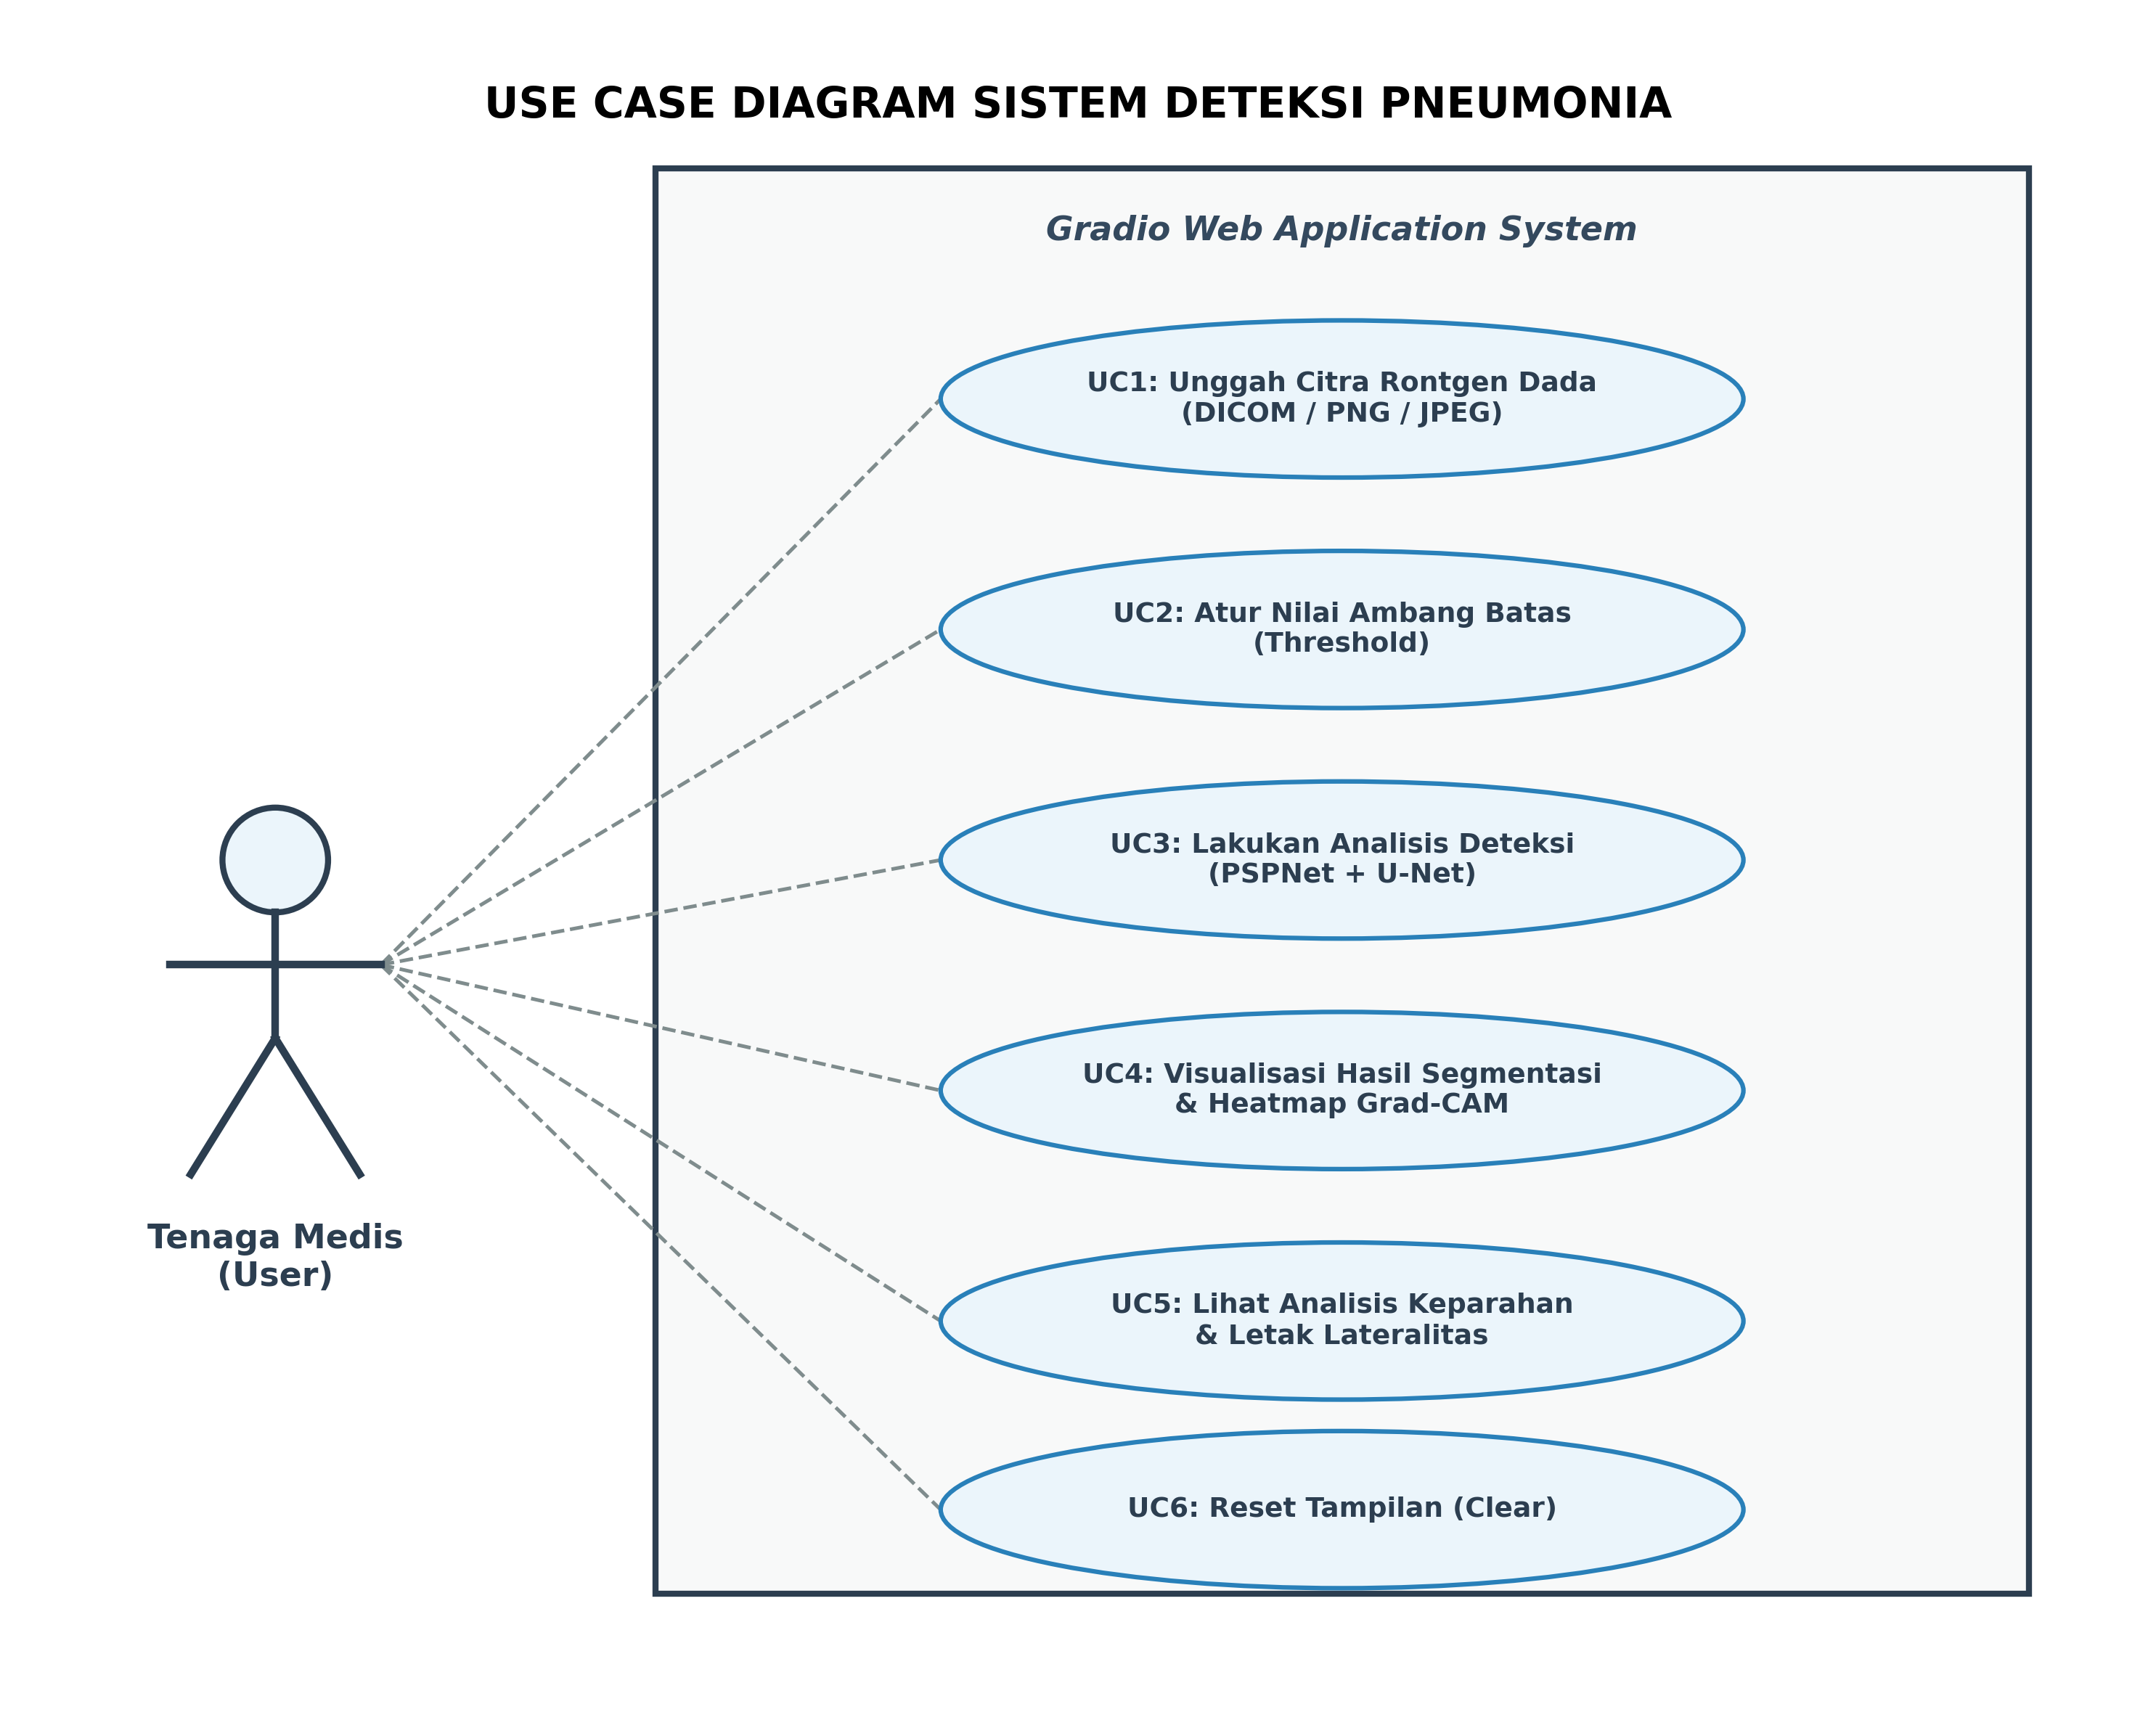
\includegraphics[width=\linewidth,height=0.7\textheight,keepaspectratio]{gambar/usecase_diagram.png}
\caption{Use Case Diagram Sistem NiagaNow}
\label{fig:usecase}
\end{figure}

\textbf{\textit{Activity} Diagram.} Diagram aktivitas menggambarkan rangkaian proses interaksi setiap peran pengguna dengan sistem. Alur pembeli dimulai dari menjelajahi produk, menambahkan item ke keranjang, validasi stok saat \textit{checkout}, hingga pembayaran melalui gerbang eksternal. Alur penjual mencakup pengelolaan produk, pemrosesan pesanan, dan pembaruan status pengiriman. Alur admin meliputi pemantauan transaksi, pengelolaan pengguna, dan verifikasi rekonsiliasi.

% TODO: Tambahkan gambar activity diagram login
\begin{figure}[H]
\centering
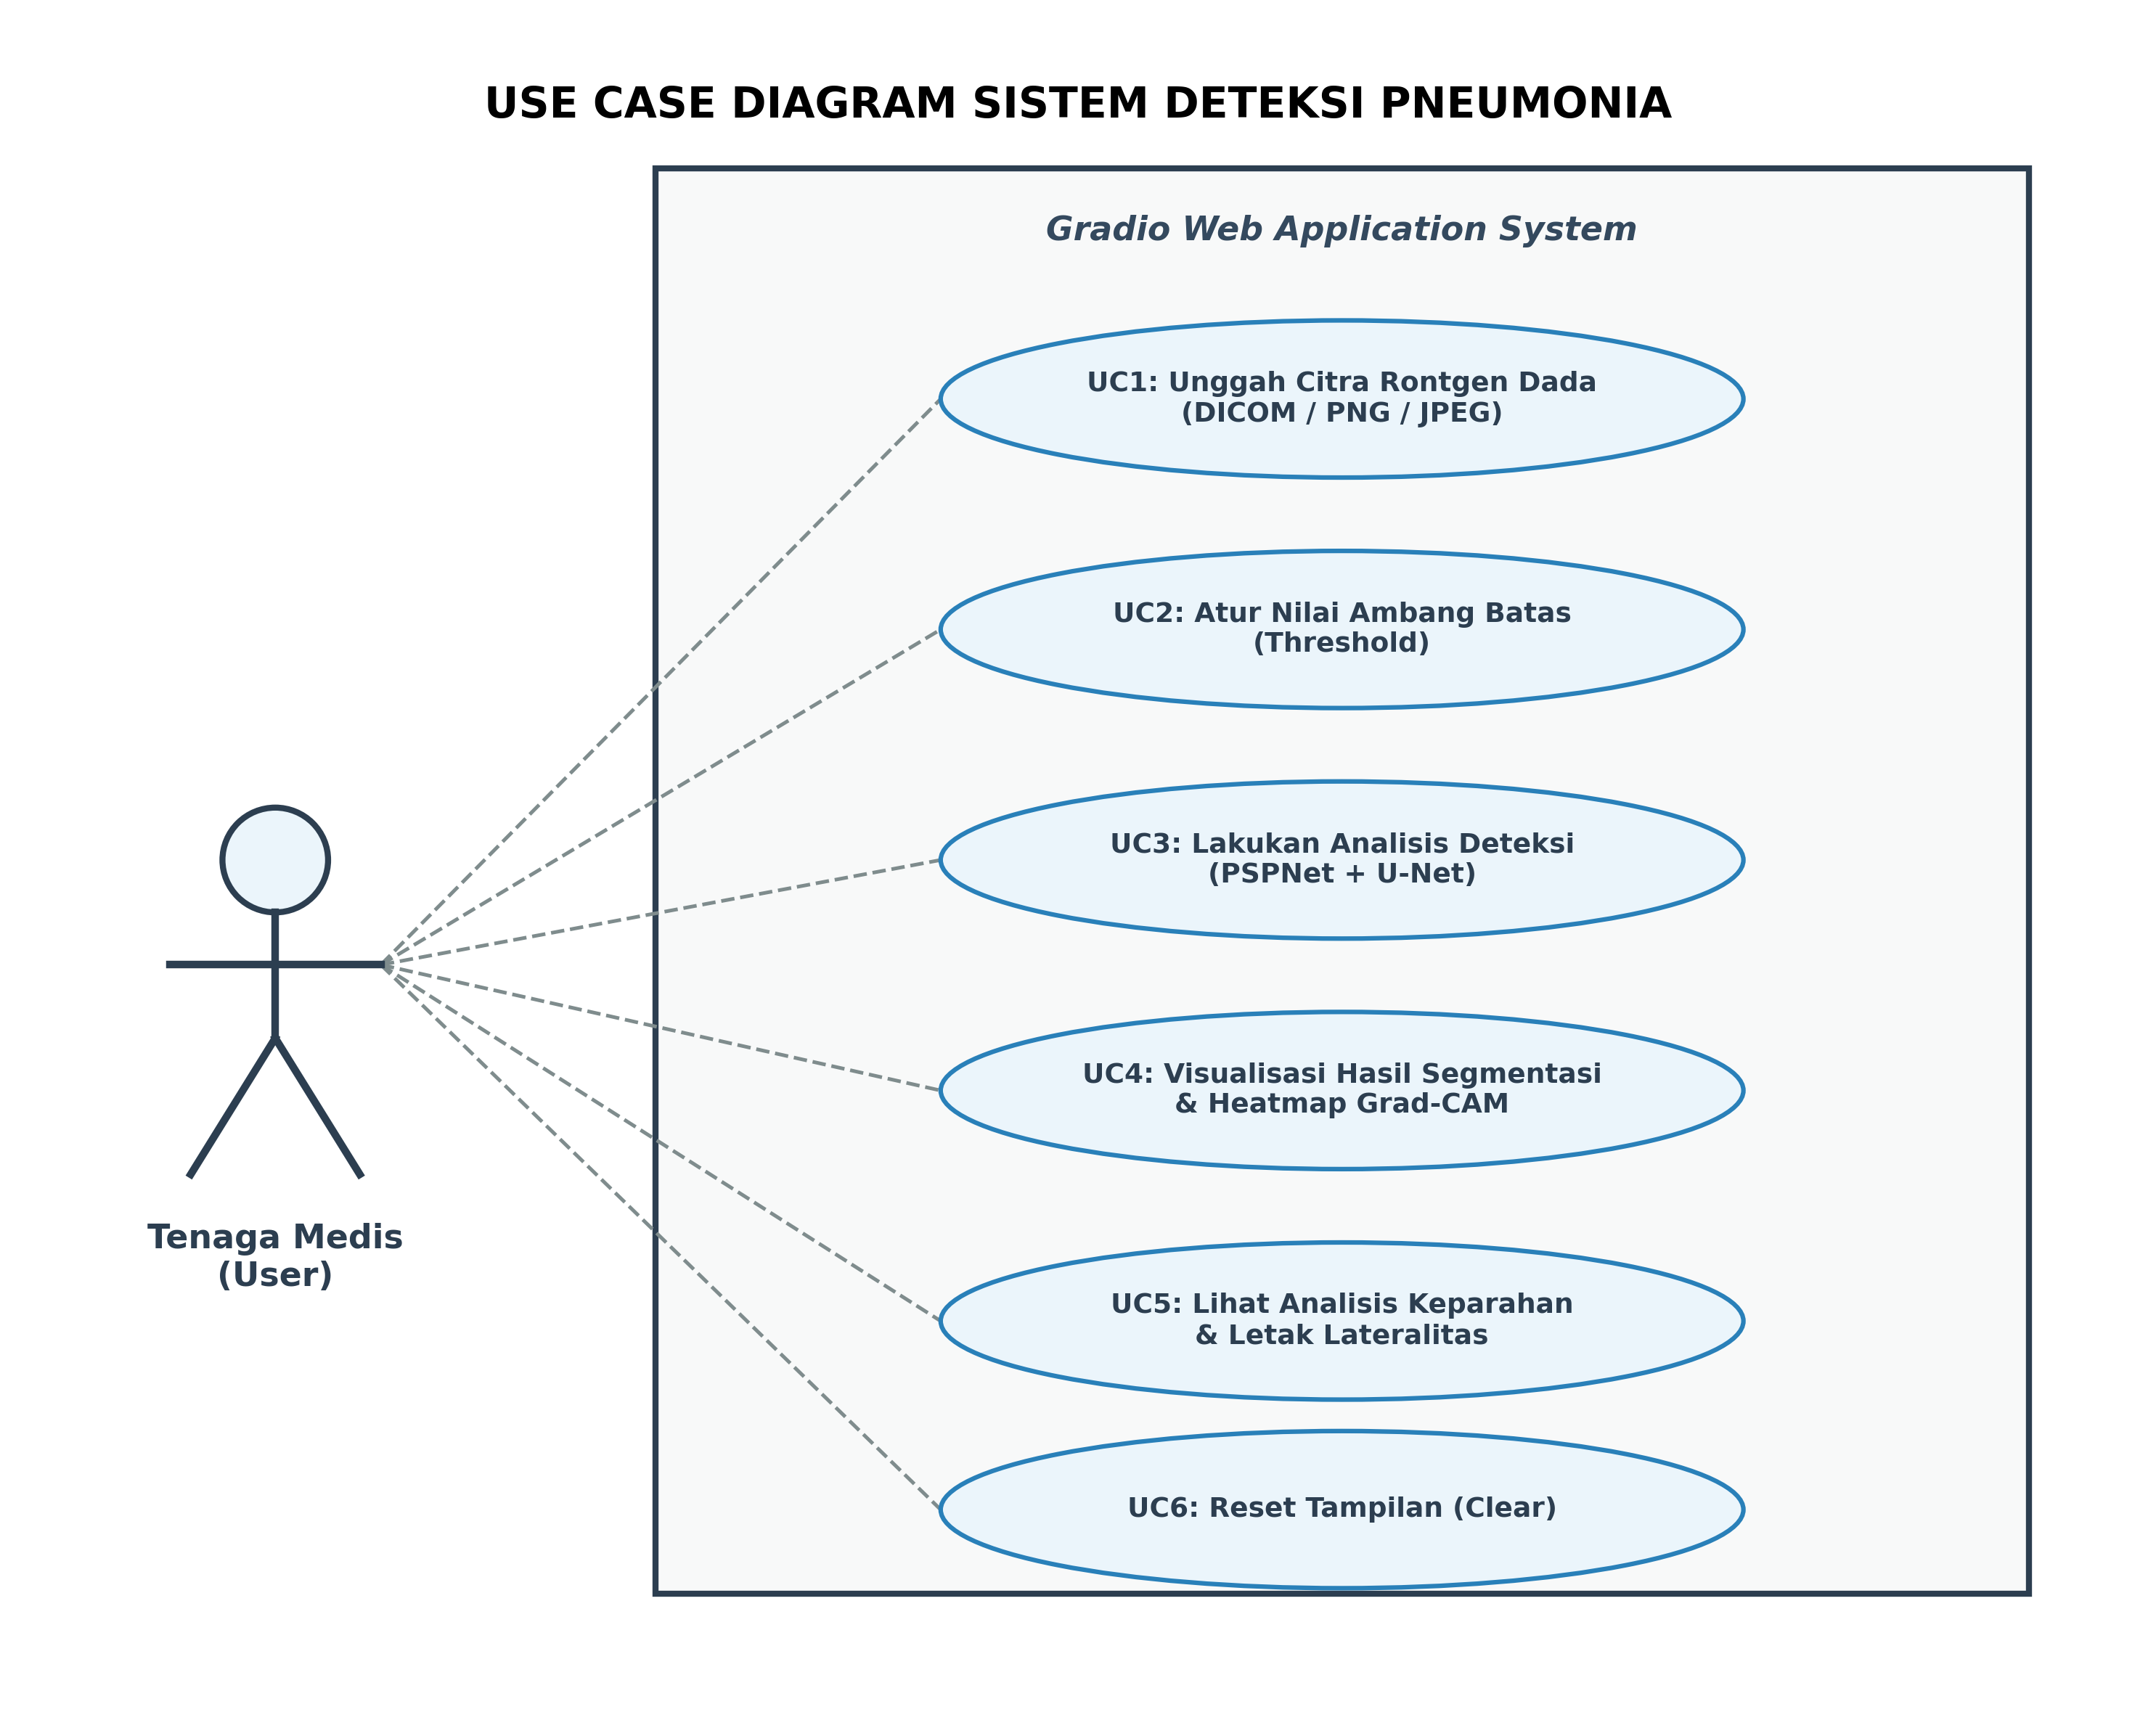
\includegraphics[width=\linewidth]{gambar/activity_login.png}
\caption{Activity Diagram Login User, Seller, Admin}
\label{fig:act_login}
\end{figure}


\textbf{\textit{Class} Diagram.} \textit{Class diagram} digunakan untuk memvisualisasikan struktur statis sistem, menggambarkan kelas-kelas utama beserta atribut dan hubungan antar kelas seperti asosiasi, agregasi, dan komposisi.

% TODO: Tambahkan gambar class diagram
\begin{figure}[H]
\centering
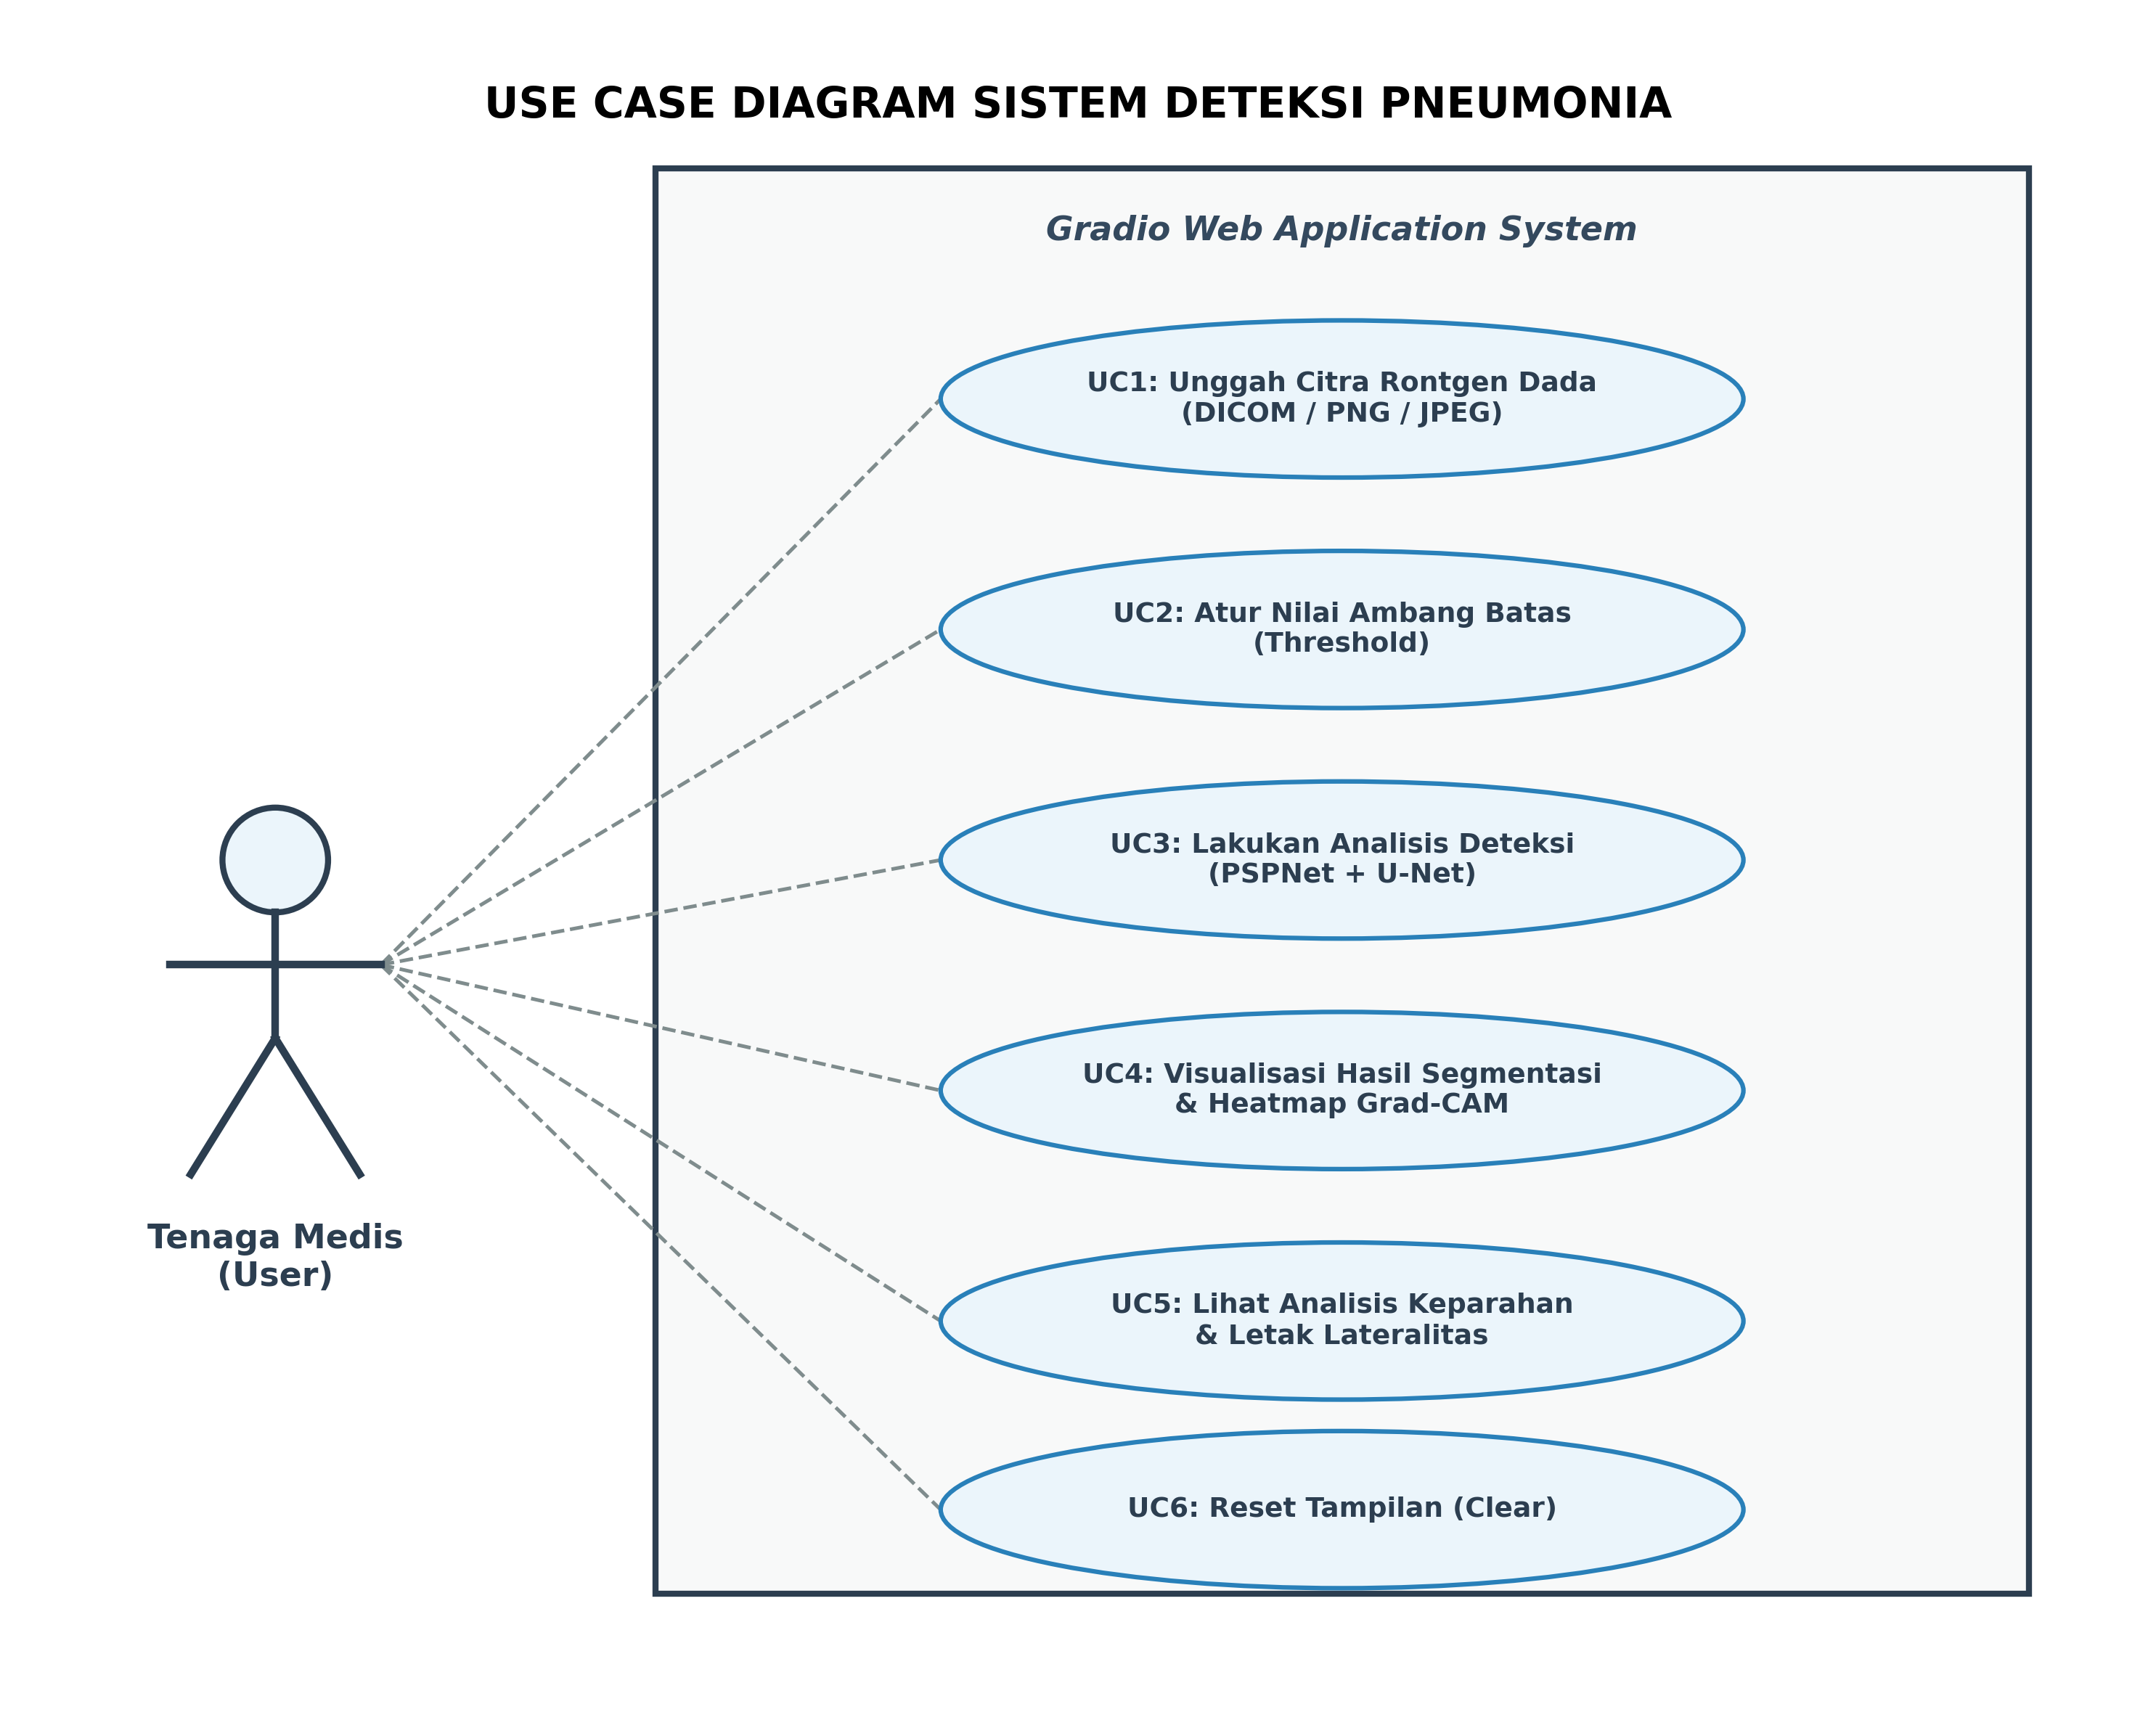
\includegraphics[width=\linewidth]{gambar/class_diagram.png}
\caption{Class Diagram Sistem NiagaNow}
\label{fig:class_diagram}
\end{figure}

\subsection{Perancangan Basis Data}

Sistem menggunakan PostgreSQL sebagai RDBMS karena keandalannya dalam menangani transaksi kompleks dengan dukungan \textit{indexing}, \textit{constraint integrity}, dan kemampuan relasional yang kuat. Implementasi dijalankan melalui kontainerisasi dengan Docker.

Basis data terdiri dari delapan tabel utama. Tabel \textit{Users} menyimpan data pengguna dengan 11 \textit{field} meliputi identitas, kredensial, dan peran. Tabel \textit{Products} menyimpan data produk dari berbagai penjual dengan 20 \textit{field} yang mencakup informasi detail produk, dimensi, garansi, dan relasi ke toko. Tabel \textit{Address} menyimpan data alamat pengguna dengan relasi \textit{many-to-one} ke \textit{Users}.

Tabel \textit{Transactions} merekam data inti transaksi dengan 18 \textit{field}, mencakup referensi pembayaran, status, total, pajak, informasi pengiriman, serta \textit{timestamp} siklus pembayaran. Tabel \textit{Orders} merepresentasikan detail pesanan per toko dalam satu transaksi dengan relasi \textit{many-to-one} ke \textit{Transactions}, \textit{Users}, dan \textit{Stores}. Tabel \textit{OrderItems} menyimpan \textit{snapshot} data produk yang dibeli sebagai salinan saat pemesanan.

Tabel \textit{Carts} merepresentasikan keranjang belanja per toko milik pengguna, sedangkan tabel \textit{CartItems} menyimpan data produk dalam keranjang beserta \textit{price\_snapshot} untuk menjaga konsistensi harga saat item dimasukkan.

\subsection{Implementasi Sistem}

Dalam pengembangan sistem marketplace \textit{e-commerce} ini, digunakan beberapa teknologi modern yang saling terintegrasi untuk mendukung kebutuhan sistem dari sisi fungsionalitas, performa, dan kemudahan pengelolaan. Teknologi-teknologi ini dipilih karena sesuai dengan kebutuhan sistem yang mendukung transaksi \textit{multi-seller}, pemrosesan banyak pesanan dalam satu transaksi (\textit{multi-order}), serta integrasi dengan layanan pembayaran Xendit.

\subsection{Pembuatan Backend}

Untuk bagian \textit{backend}, digunakan Spring Boot karena \textit{framework} ini sangat cocok dalam membangun API berbasis REST secara cepat dan efisien. Spring Boot sudah menyediakan banyak fitur bawaan seperti manajemen \textit{database}, pengelolaan transaksi, serta dukungan pengamanan API. Selain itu, Spring Boot juga sangat fleksibel untuk terhubung dengan layanan eksternal seperti Xendit melalui konfigurasi HTTP \textit{client}. Dengan menggunakan Spring Boot, proses pengembangan \textit{backend} menjadi lebih cepat dan terstruktur, serta memudahkan dalam pengujian dan \textit{deployment}.

% TODO: Tambahkan gambar Spring Initializr
\begin{figure}[H]
\centering
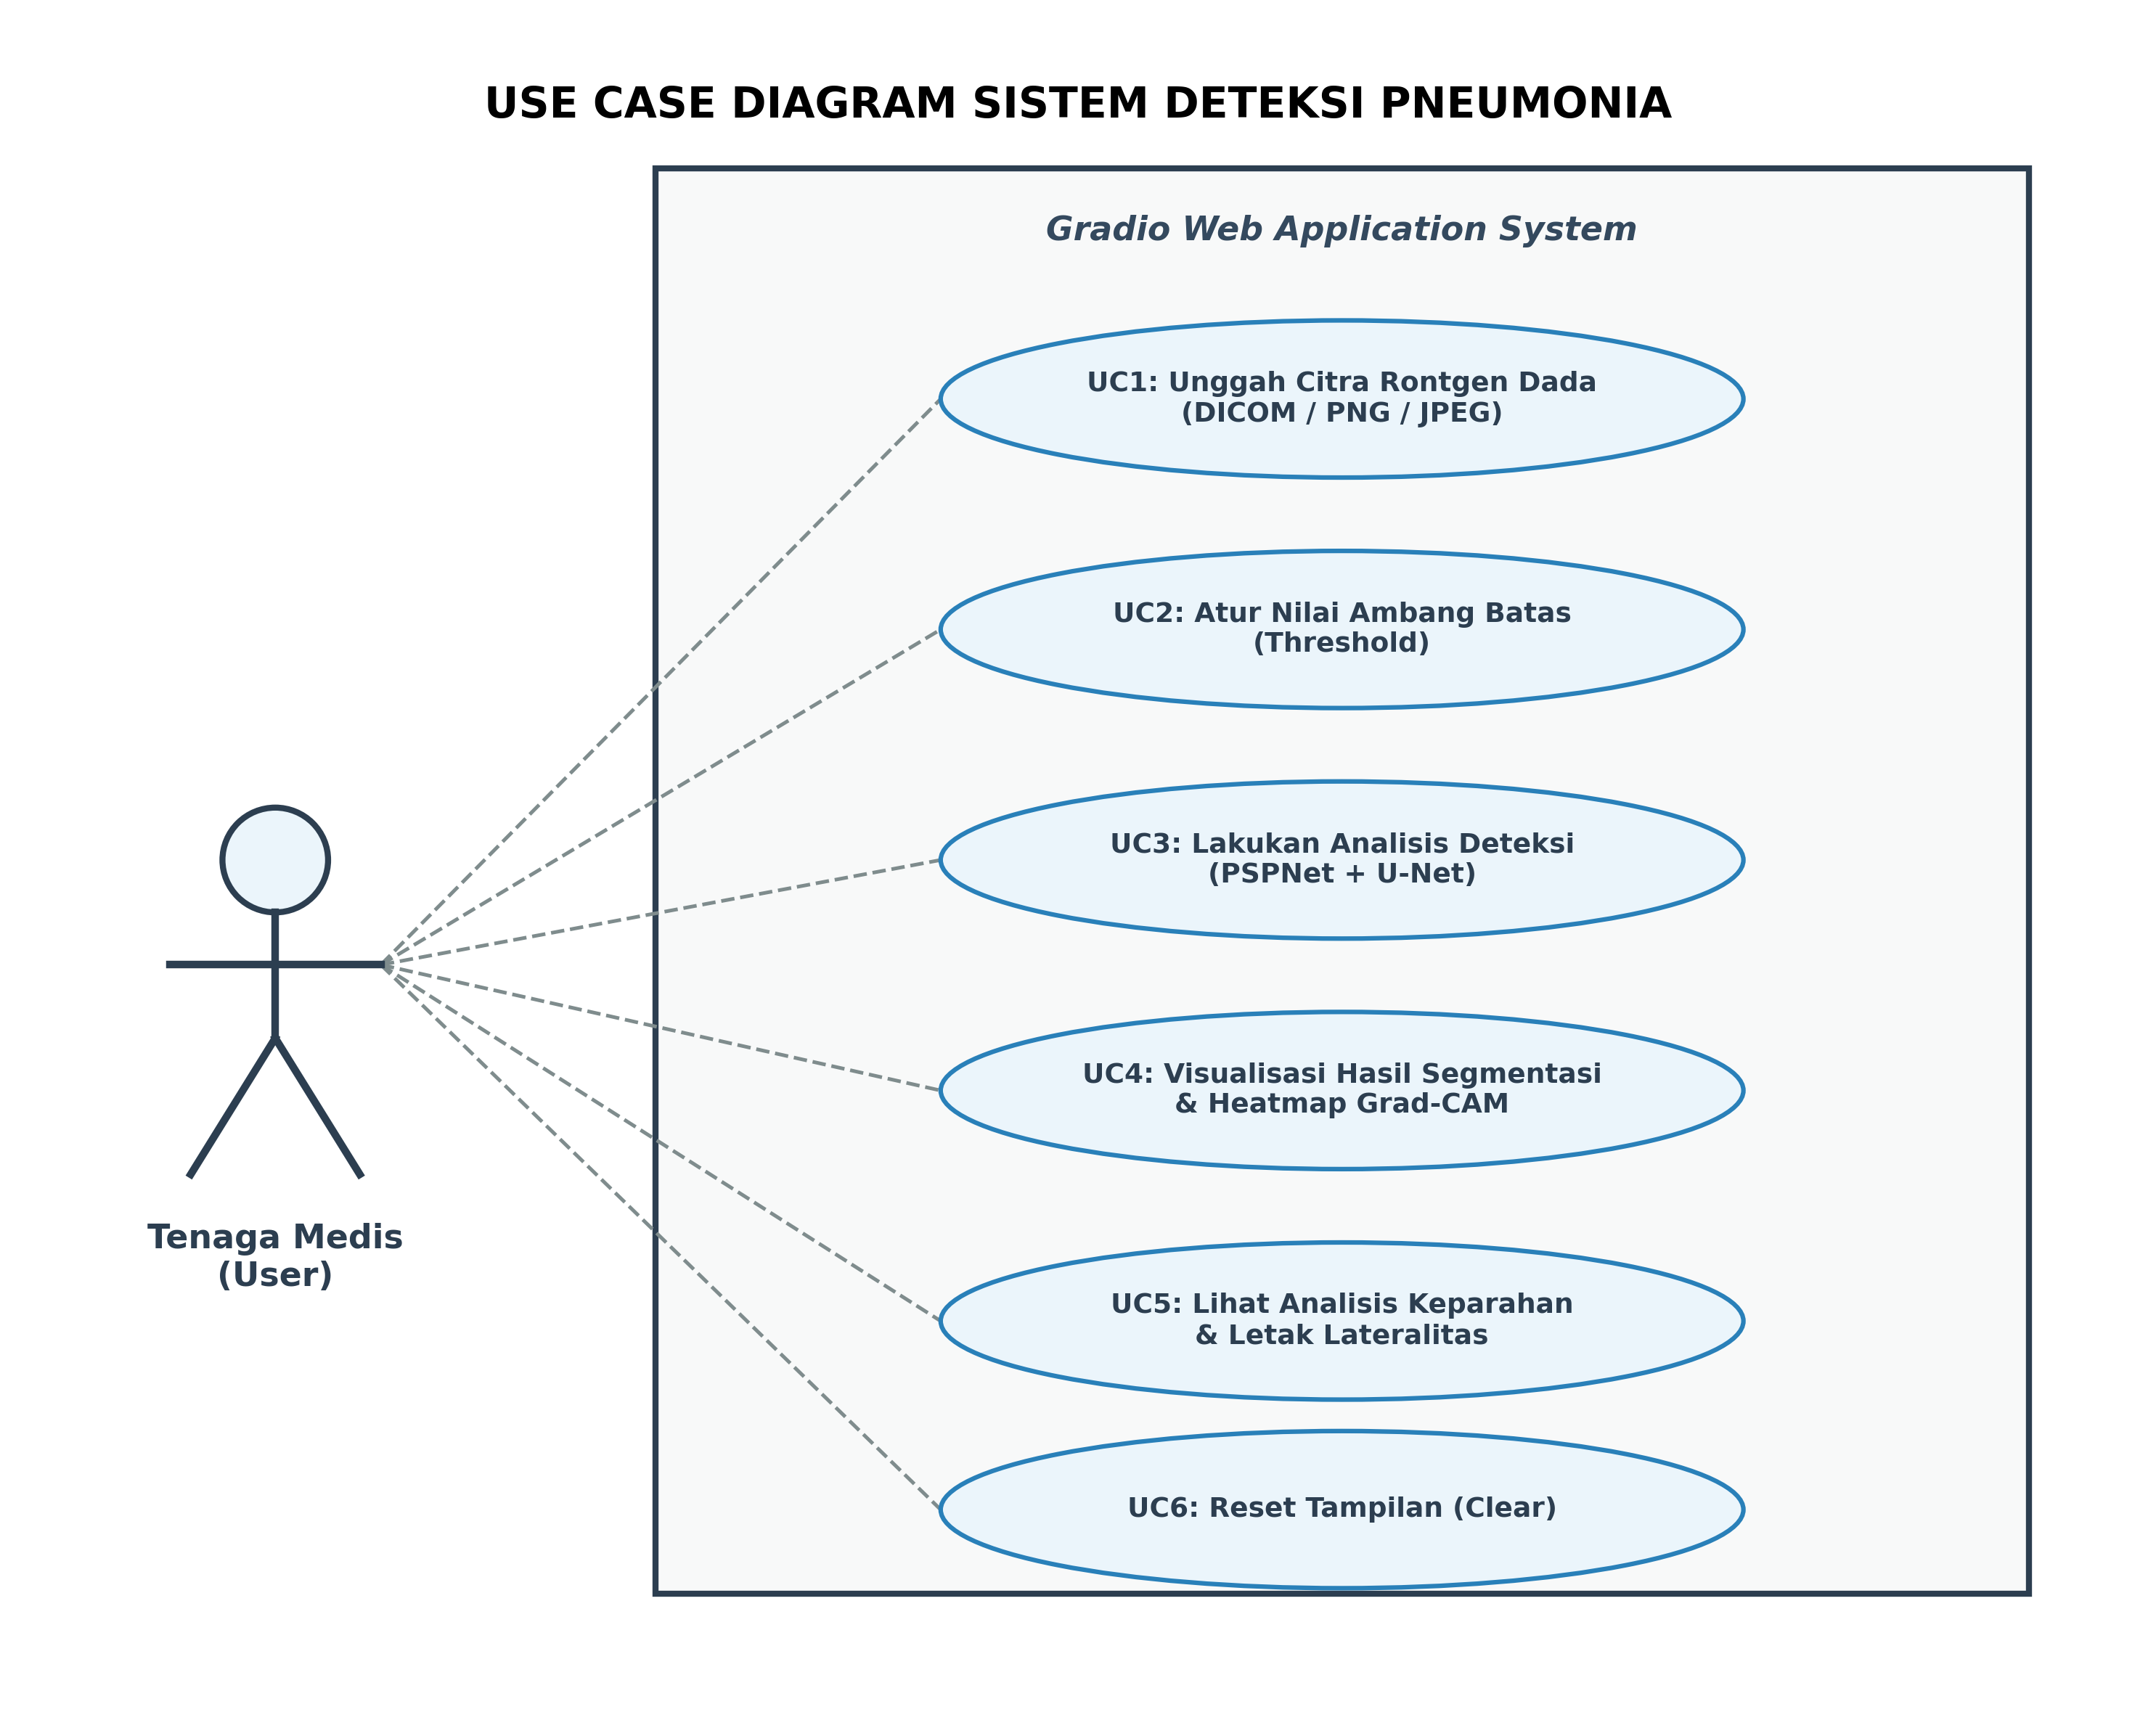
\includegraphics[width=\linewidth]{gambar/spring_initializr.png}
\caption{Spring Initializr}
\label{fig:spring_initializr}
\end{figure}

\textbf{Implementasi Logika Layanan Pengguna.} Kelas \texttt{UserService} bertanggung jawab untuk menangani logika bisnis yang berkaitan dengan pengelolaan pengguna (\textit{user management}) dalam sistem \textit{e-commerce} EzyShop. Komponen ini diimplementasikan sebagai bagian dari lapisan \textit{service} pada arsitektur berorientasi layanan (\textit{service-oriented architecture}) menggunakan \textit{framework} Spring Boot.

Kelas ini mengimplementasikan antarmuka \texttt{UserDetailsService} dari Spring Security, yang memungkinkan sistem melakukan autentikasi pengguna berdasarkan nama pengguna (\textit{username}). Dalam metode \texttt{loadUserByUsername}, sistem memuat detail pengguna yang dibungkus dalam objek \texttt{UserDetailsImpl}. Apabila pengguna tidak ditemukan dalam basis data, maka akan dilemparkan pengecualian \texttt{UsernameNotFoundException}.

Untuk keperluan registrasi pengguna, metode \texttt{registerUser} menerima parameter berupa nama pengguna, kata sandi mentah (\textit{raw password}), email, dan nama lengkap. Proses registrasi mencakup validasi eksistensi nama pengguna dan email, serta enkripsi kata sandi menggunakan \texttt{PasswordEncoder}. Jika semua validasi berhasil, data pengguna akan disimpan ke dalam repositori.

Untuk autentikasi login, metode \texttt{loginUser} memastikan bahwa kombinasi nama pengguna dan kata sandi valid. Pengambilan data profil pengguna dilakukan melalui metode \texttt{getUserProfile}, yang mengonversinya ke DTO (\texttt{ProfileDto}) dengan bantuan \texttt{UserMapper}. Kelas ini juga mengakomodasi penghapusan pengguna secara permanen (\textit{hard delete}) melalui metode \texttt{deleteUser}, maupun secara sementara (\textit{soft delete}) melalui metode \texttt{disableUser}.

Sebagai bagian dari sistem marketplace multi-penjual, \texttt{UserService} menyediakan fitur peningkatan akun pengguna menjadi penjual melalui metode \texttt{upgradeToSeller}. Fitur ini memverifikasi kesesuaian nama pengguna dan sandi, memastikan nama toko bersifat unik, dan membentuk entitas \texttt{Store} yang terasosiasi dengan pengguna. Penomoran toko dilakukan secara otomatis menggunakan metode \texttt{generateStoreNo}, yang menghasilkan nomor toko unik dalam format \texttt{STXXXX}.

\textbf{Implementasi Logika Autentikasi dan Otorisasi.} Kelas \texttt{AuthController} merupakan komponen pengendali utama yang menangani permintaan terkait proses autentikasi, otorisasi, serta pengelolaan identitas pengguna pada sistem EzyShop. Kelas ini diimplementasikan menggunakan anotasi \texttt{@RestController} dan menangani permintaan HTTP di bawah jalur \texttt{/api/v1/auth}.

Metode \texttt{login} digunakan untuk memverifikasi kredensial pengguna. Proses ini dimulai dengan otentikasi melalui \texttt{UserService}, kemudian sistem menghasilkan token \textit{refresh} berbasis JWT (\textit{JSON Web Token}). Token ini disimpan dalam repository Redis guna validasi sesi dan disisipkan ke dalam \textit{cookie} HTTP-only untuk alasan keamanan.

Metode \texttt{register} menerapkan proses pendaftaran pengguna baru. Sistem juga langsung membuat token \textit{refresh} baru bagi pengguna yang baru terdaftar. Pada metode \texttt{upgradeToSeller}, pengguna yang telah login dapat mengajukan peningkatan peran menjadi penjual. Metode \texttt{refresh} digunakan untuk menghasilkan token akses baru menggunakan token \textit{refresh} yang masih valid. Metode \texttt{validate} disediakan untuk mengecek validitas token akses. Metode \texttt{getProfile} dan \texttt{updateProfile} memungkinkan pengguna untuk membaca dan memperbarui informasi profil. Fungsi \texttt{logout} bertugas untuk menghapus token \textit{refresh} dari Redis dan mengosongkan \textit{cookie} pada sisi klien.

\textbf{Implementasi \textit{Payment Gateway} dengan Xendit.} Implementasi layanan pembayaran memungkinkan pengguna untuk melakukan transaksi menggunakan berbagai metode pembayaran seperti \textit{e-wallet} (DANA, GoPay) dan \textit{virtual account} bank (BCA VA).

Program ini dirancang untuk menangani permintaan pembayaran dari pengguna dengan memanfaatkan API eksternal Xendit. Setiap permintaan pembayaran diterima dalam bentuk objek \texttt{PaymentRequest} yang berisi informasi seperti detail keranjang belanja, alamat pengiriman, pajak, dan metode pembayaran yang dipilih.

Fungsi \texttt{handlePayment} melakukan beberapa langkah penting. Pertama, ia mengonversi data permintaan pembayaran menjadi format yang sesuai dengan metode pembayaran yang dipilih menggunakan \textit{mapper} khusus seperti \texttt{MapperEWallet} atau \texttt{MapperBank}. Selanjutnya, program mengirimkan permintaan HTTP POST ke \textit{endpoint} API Xendit untuk memproses pembayaran. Setelah menerima respons dari Xendit, program membuat entitas transaksi baru yang mencakup informasi seperti ID referensi, status pembayaran, pajak, biaya pengiriman, dan detail tindakan lebih lanjut.

\textit{Webhook} adalah mekanisme yang digunakan oleh Xendit untuk memberi tahu sistem internal tentang perubahan status transaksi. Kontroler \texttt{XenditWebhookController} dirancang untuk menerima notifikasi dari Xendit melalui \textit{endpoint} HTTP POST. Salah satu fungsi utama kontroler ini adalah memverifikasi keaslian notifikasi yang diterima dengan membandingkan \textit{token callback} yang dikirimkan oleh Xendit dengan nilai rahasia yang telah ditentukan sebelumnya. Setelah verifikasi berhasil, program memproses \textit{payload} notifikasi secara asinkron menggunakan layanan \texttt{WebhookService}.

\subsection{Pembuatan Frontend}

Pembuatan antarmuka pengguna (\textit{frontend}) NiagaNow dilakukan menggunakan SolidJS, sebuah \textit{framework} JavaScript modern yang mengedepankan reaktivitas tanpa \textit{virtual} DOM. Struktur \textit{frontend} dikembangkan dengan pendekatan komponen berbasis halaman, meliputi halaman utama, daftar produk, detail produk, \textit{checkout}, serta akun pengguna. Untuk pengelolaan \textit{routing} antar halaman digunakan \texttt{@tanstack/solid-router}, sedangkan pengambilan dan sinkronisasi data dari \textit{backend} ditangani oleh \texttt{@tanstack/query}.

Desain antarmuka mengikuti prinsip \textit{mobile-first} dan \textit{user-centered design}. Proses desain diawali dengan penyusunan \textit{mockup} di Figma, yang kemudian diterjemahkan secara iteratif menggunakan Tailwind CSS. Aplikasi \textit{frontend} dikemas menggunakan Vite dan disajikan sebagai \textit{Single Page Application} (SPA), di mana seluruh navigasi ditangani di sisi klien.

% TODO: Tambahkan gambar Solid JS
\begin{figure}[H]
\centering
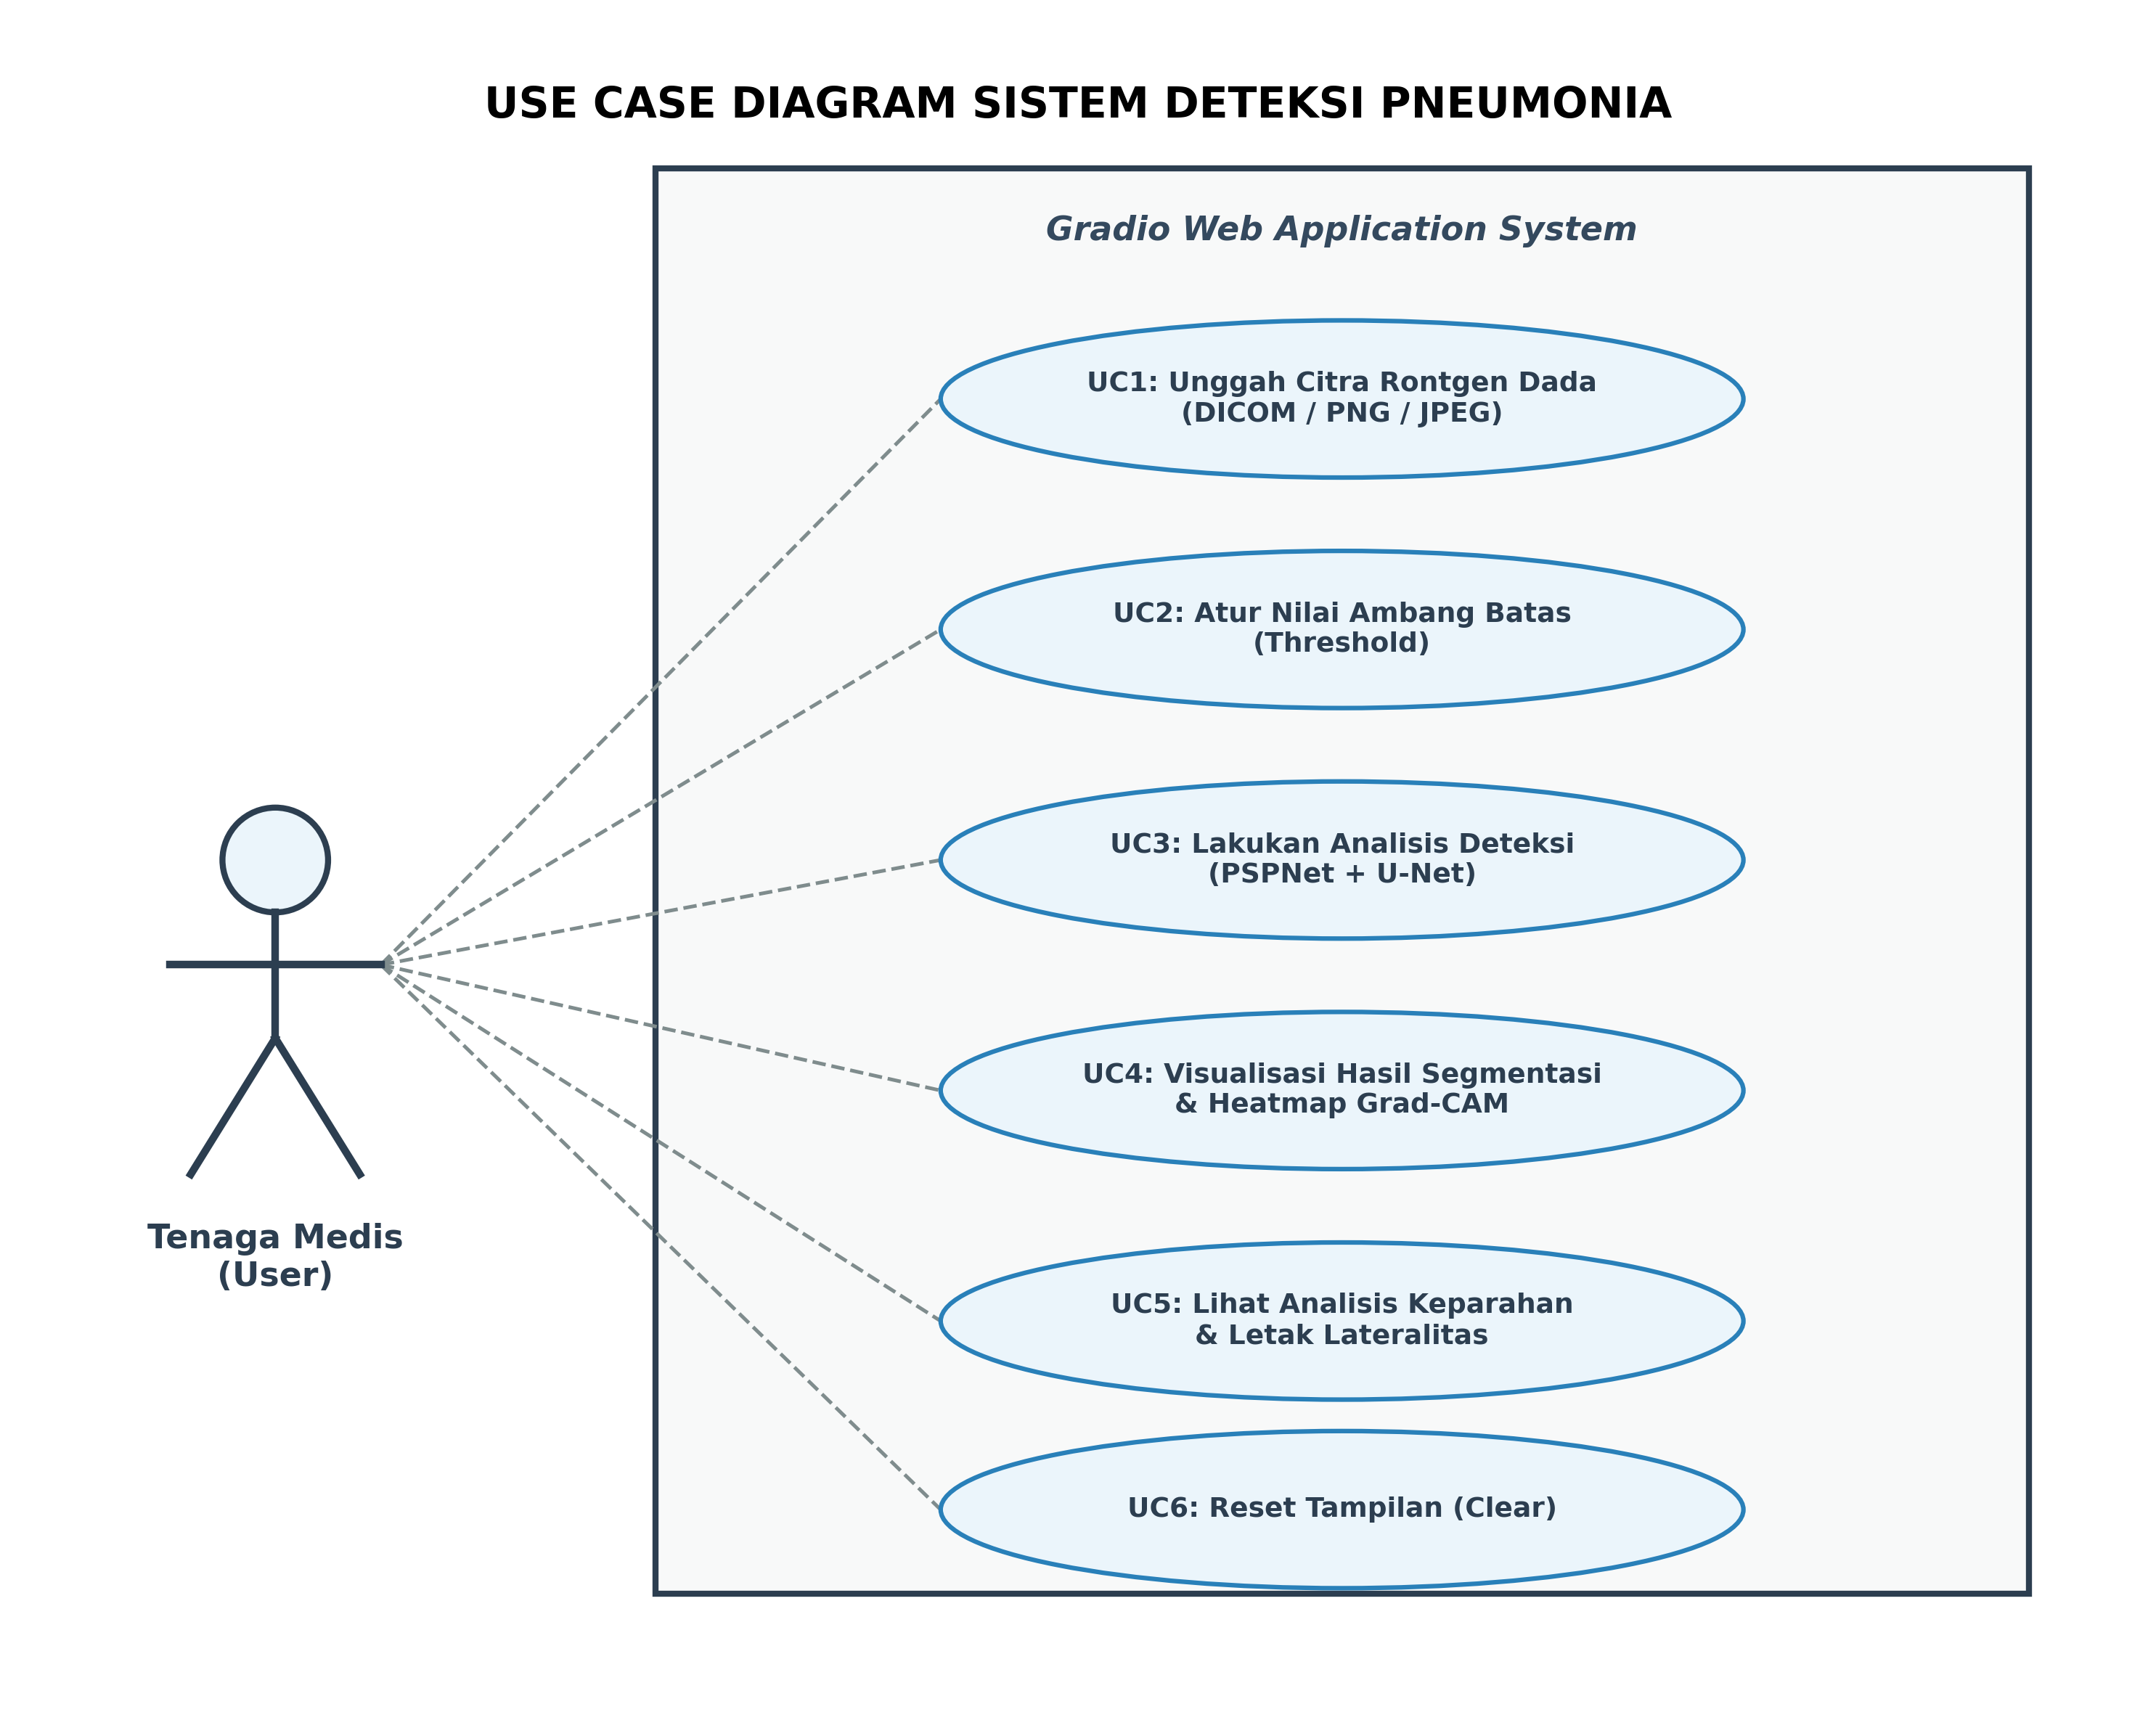
\includegraphics[width=\linewidth]{gambar/solidjs.png}
\caption{Solid JS}
\label{fig:solidjs}
\end{figure}

\textbf{Halaman Home.} Halaman beranda dirancang untuk menampilkan produk secara dinamis menggunakan SolidJS dan TanStack Query. Data produk diambil menggunakan fungsi \texttt{getProducts} melalui \textit{hook} \texttt{useQuery} dengan dukungan \textit{caching}, \textit{prefetching}, dan status \textit{loading}.

\textbf{Halaman Products.} Halaman produk menampilkan daftar produk secara dinamis dengan integrasi fitur filter, \textit{pagination}, dan \textit{lazy loading}. Validasi parameter pencarian dilakukan menggunakan fungsi \texttt{validateSearch} dan \textit{prefetching} data dilakukan melalui \textit{loader route}.

\textbf{Halaman Product Detail.} Halaman produk detail menampilkan informasi spesifik tentang sebuah produk berdasarkan ID, termasuk deskripsi, harga, gambar, ulasan, dan opsi pembelian. Fungsionalitas penambahan produk ke keranjang diimplementasikan menggunakan \textit{hook} \texttt{useMutation}.

\textbf{Halaman My-Orders.} Halaman ini menampilkan daftar pesanan pengguna yang terautentikasi. Data pesanan diambil menggunakan \texttt{useQuery} yang memanggil fungsi \texttt{getOrders} dengan token autentikasi sebagai parameter.

\textbf{Halaman Address.} Halaman pengelolaan alamat memungkinkan pengguna mengelola informasi alamat secara dinamis, termasuk menambahkan, menghapus, dan memperbarui alamat. Setiap operasi diimplementasikan menggunakan \textit{hook} \texttt{useMutation}.

\textbf{Halaman Sign Up.} Halaman pendaftaran memungkinkan pengguna membuat akun baru. Data formulir dikelola menggunakan \texttt{createStore} dan proses pengiriman data dilakukan menggunakan \texttt{useMutation} dari TanStack Query.

\textbf{Halaman Login.} Halaman login memungkinkan pengguna melakukan autentikasi. Proses autentikasi dilakukan menggunakan \texttt{useMutation} yang memanggil fungsi \texttt{postLoginUser}.

\textbf{Halaman Logout.} Halaman logout memungkinkan pengguna mengakhiri sesi autentikasi dengan aman. Proses ini melibatkan penghapusan data otentikasi dari konteks aplikasi dan mengarahkan pengguna kembali ke halaman login.

\textbf{Halaman Cart.} Halaman keranjang belanja memberikan pengalaman interaktif dalam mengelola item-item yang telah ditambahkan ke keranjang. Fungsionalitas utama mencakup menambah/mengurangi jumlah item, menghapus item, dan memilih item untuk \textit{checkout}.

\textbf{Halaman Checkout.} Halaman \textit{checkout} memungkinkan pengguna menyelesaikan proses pembelian dengan memilih metode pembayaran, alamat pengiriman, dan jenis pengiriman. Pengguna dapat memilih metode pembayaran seperti \textit{virtual account} atau \textit{e-wallet}.

\textbf{Halaman Order Details.} Halaman detail pesanan memberikan informasi lengkap mengenai status transaksi berdasarkan ID referensi. Halaman ini memungkinkan pengguna untuk melihat status pembayaran, mencetak detail transaksi, dan melakukan pengecekan ulang status pembayaran secara dinamis.

\textbf{Halaman Store Dashboard.} Halaman ini menampilkan data pesanan dan produk yang terkait dengan toko pengguna yang sedang login. Data diambil menggunakan fungsi \texttt{getOrdersByStoreIdLimit} dan \texttt{getProductsByStoreId}.

\textbf{Halaman Store Orders.} Halaman ini menampilkan daftar pesanan toko dengan ringkasan statistik seperti total pesanan, total pendapatan, dan rata-rata nilai pesanan. Fungsionalitas filter pesanan diimplementasikan menggunakan \textit{memoized value}.

\textbf{Halaman Store Products.} Halaman ini mengelola data produk dalam konteks toko dengan fitur filtrasi berdasarkan status produk serta operasi penghapusan dan pengaktifan produk.

\textbf{Halaman Add Products.} Halaman ini menyediakan antarmuka untuk menambahkan produk baru, termasuk informasi dasar, kategori, gambar, dan \textit{thumbnail} produk. Proses unggah gambar dilakukan melalui \texttt{useMutation} dengan \texttt{FormData}.

\textbf{Halaman Update Product.} Halaman ini memungkinkan pengguna memperbarui produk di toko mereka, termasuk detail dasar, kategori, gambar, dan \textit{thumbnail}.

\textbf{Halaman Admin Dashboard.} Halaman \textit{dashboard} admin memberikan gambaran menyeluruh tentang data operasional platform, mencakup data toko, pengguna, produk, dan transaksi.

\textbf{Halaman Admin Products.} Halaman ini menyediakan antarmuka administratif untuk pengelolaan produk dengan kemampuan filtrasi berdasarkan status dan kata kunci pencarian.

\textbf{Halaman Admin Stores.} Halaman ini menyediakan antarmuka administratif untuk pengelolaan toko dengan filtrasi berdasarkan status aktif atau nonaktif.

\textbf{Halaman Admin Transactions.} Halaman ini menampilkan daftar transaksi platform dengan ringkasan statistik seperti total transaksi, total pendapatan, rata-rata nilai transaksi, dan jumlah transaksi berhasil.

\textbf{Halaman Admin Users.} Halaman ini mengelola daftar pengguna pada platform, memungkinkan admin untuk melihat, menyaring, menonaktifkan, dan mengaktifkan kembali akun pengguna.

\subsection{Pembuatan Basis Data}

Pada sisi basis data, sistem manajemen basis data menggunakan PostgreSQL yang dijalankan melalui Docker. PostgreSQL dipilih karena kemampuannya dalam menangani relasi data yang kompleks dan mendukung berbagai fitur tingkat lanjut seperti \textit{indexing}, validasi, dan kueri performa tinggi. Selain PostgreSQL, digunakan juga Redis, yang juga dijalankan di dalam kontainer Docker, sebagai penyimpanan sementara (\textit{cache}) untuk mempercepat pemrosesan data tertentu, misalnya verifikasi token JWT.

% TODO: Tambahkan gambar Docker Desktop
\begin{figure}[H]
\centering
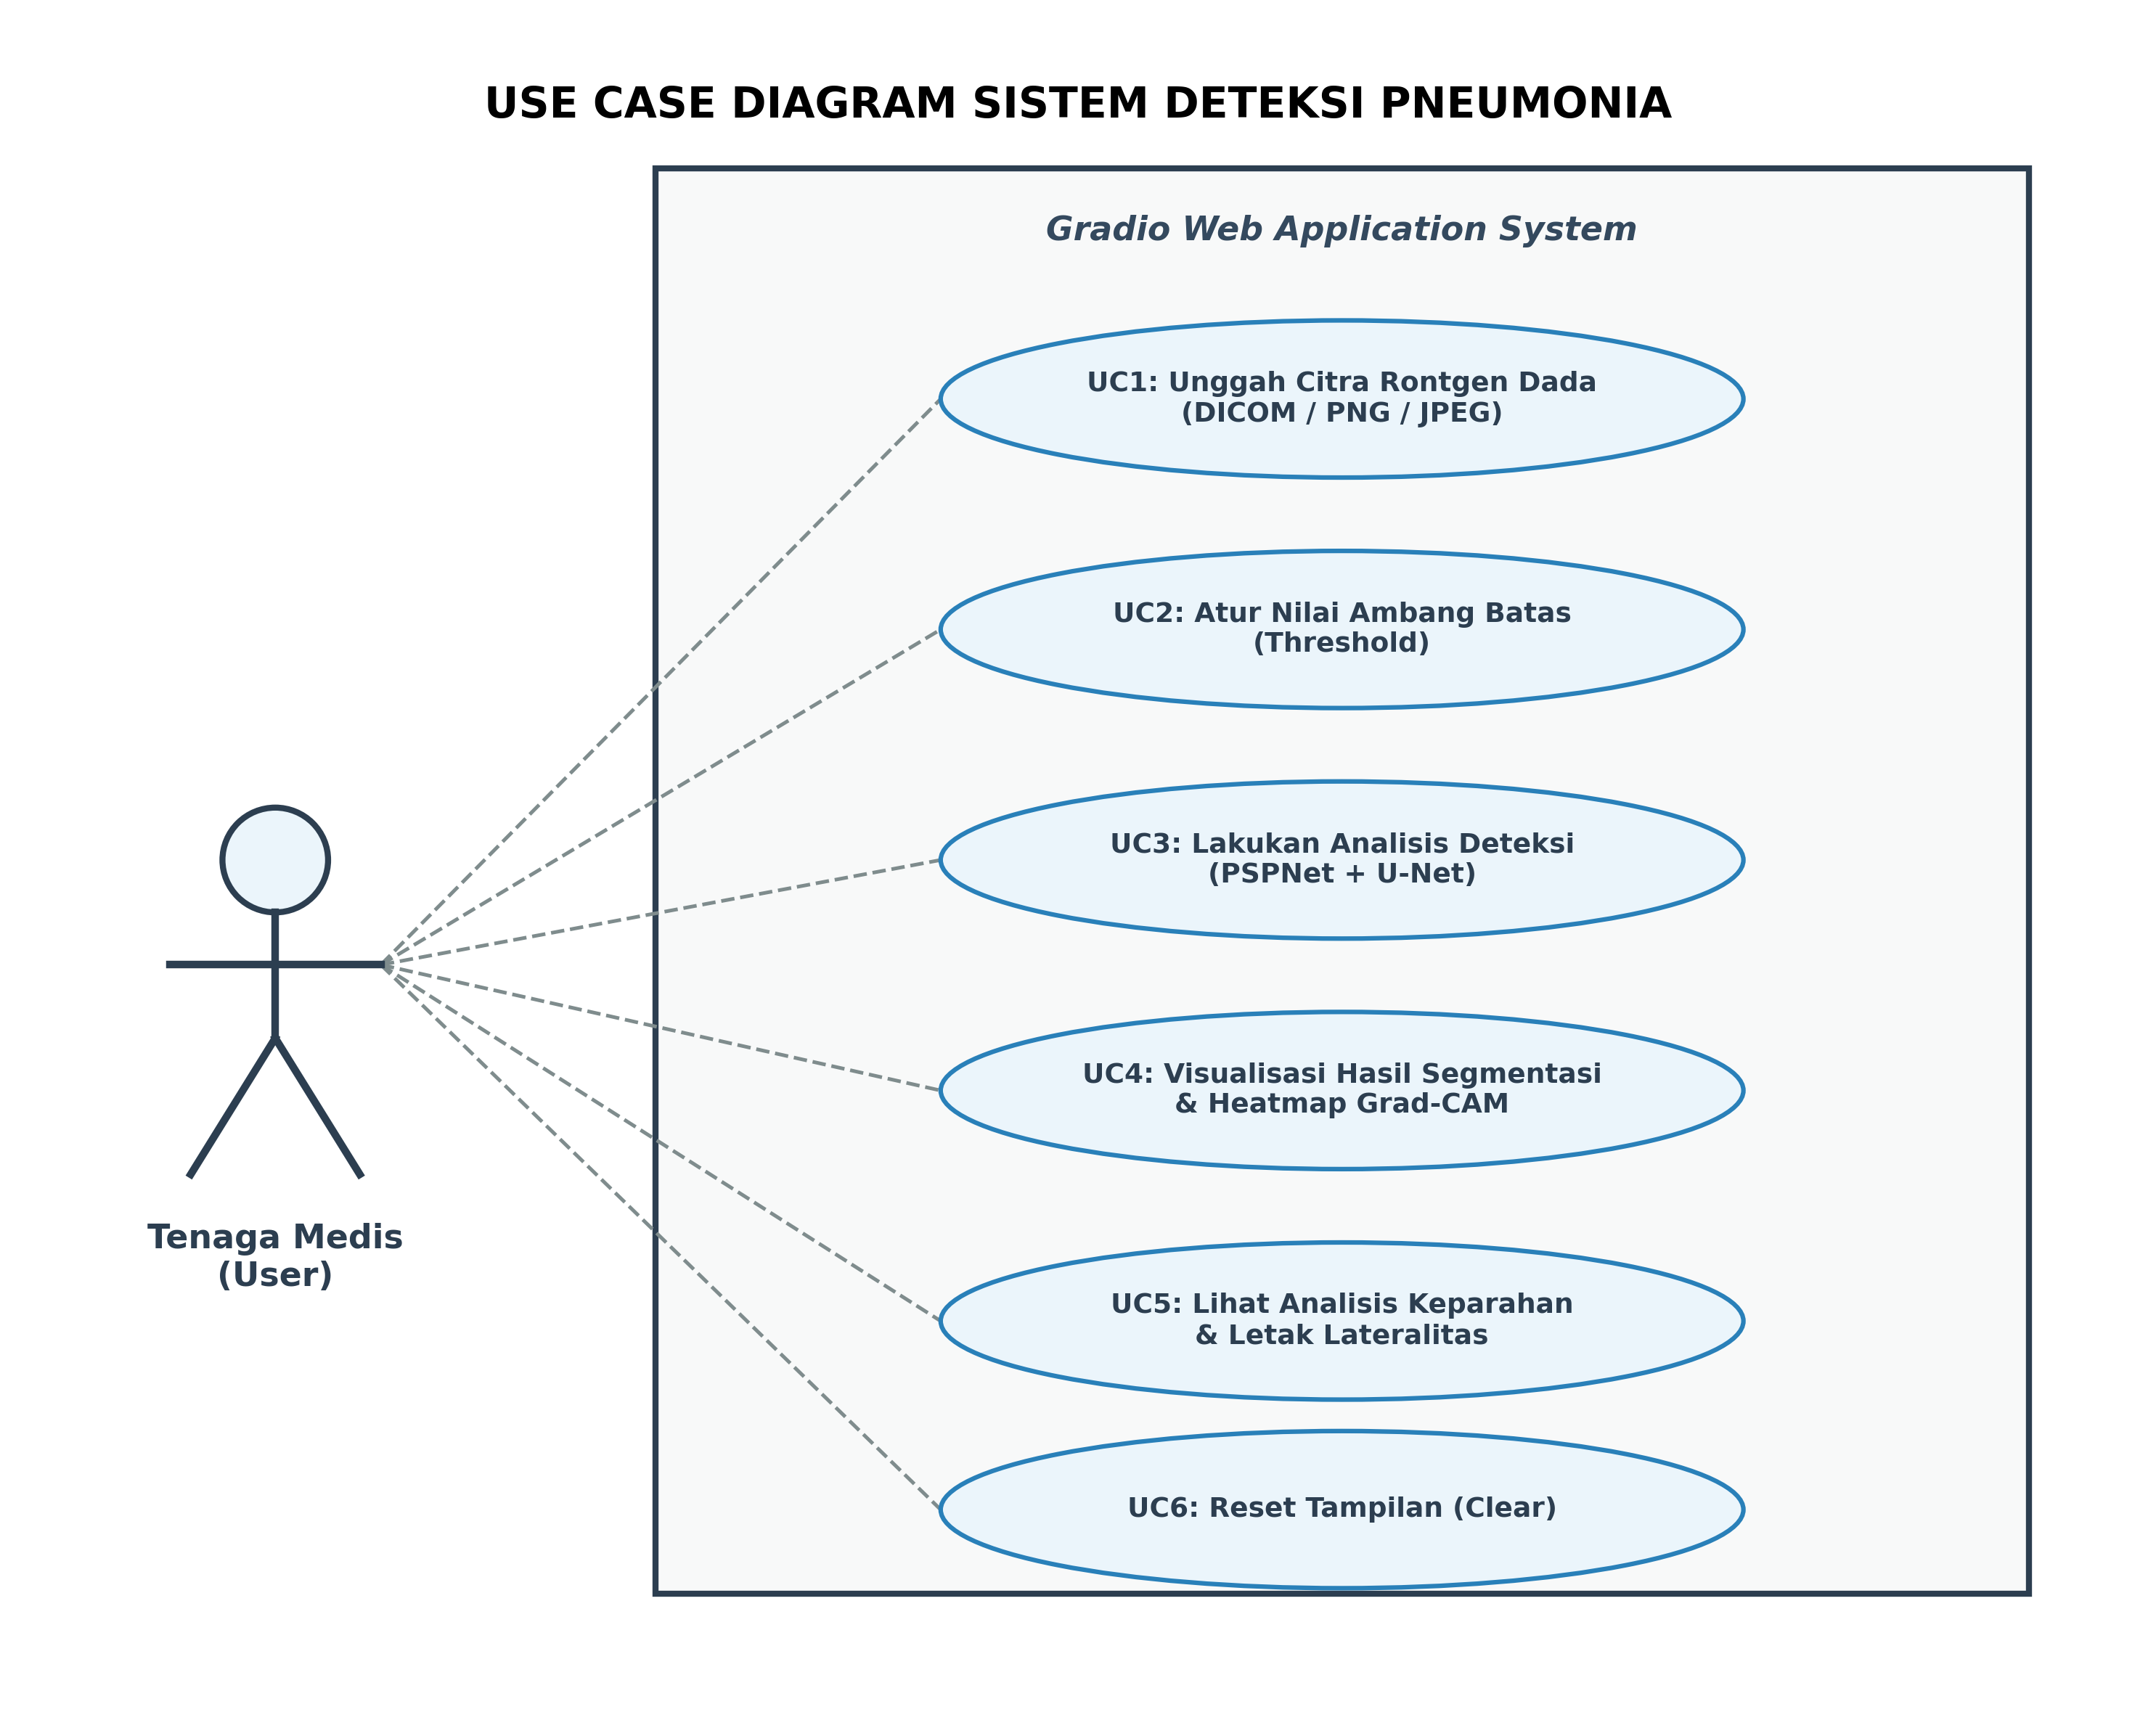
\includegraphics[width=\linewidth]{gambar/docker_desktop.png}
\caption{Docker Desktop}
\label{fig:docker_desktop}
\end{figure}

Dalam implementasinya, pembuatan dan pengelolaan tabel pada basis data PostgreSQL dilakukan secara otomatis menggunakan Spring Data JPA. Spring JPA adalah bagian dari ekosistem Spring yang memungkinkan pengembang mendefinisikan struktur tabel melalui anotasi pada kelas-kelas entitas Java. Dengan menggunakan pendekatan ini, proses pembuatan tabel menjadi lebih efisien karena cukup menuliskan definisi entitas (seperti \texttt{User}, \texttt{Store}, \texttt{Product}, \texttt{Order}, dan \texttt{Transaction}) dalam bentuk \textit{class} Java yang sudah diberi anotasi seperti \texttt{@Entity}, \texttt{@Table}, \texttt{@Id}, \texttt{@Column}, dan \texttt{@ManyToOne}.

\subsection{Uji Coba sebagai User}

Pengujian ini dilakukan menggunakan metode \textit{blackbox testing}, di mana pengujian berfokus pada fungsionalitas sistem berdasarkan \textit{input} dan \textit{output} yang tampak dari sisi pengguna. Hasil dari pengujian ini dirangkum dalam Tabel~\ref{tab:uji_user}.

\begin{table}[!ht]
\centering
\caption{Hasil Uji Coba \textit{Blackbox} sebagai User}
\label{tab:uji_user}
\resizebox{\columnwidth}{!}{
\begin{tabular}{|c|p{2cm}|p{2.5cm}|p{2.5cm}|p{2.5cm}|c|}
\hline
\textbf{No} & \textbf{Fitur} & \textbf{Langkah Uji} & \textbf{Output Diharapkan} & \textbf{Output Aktual} & \textbf{Status} \\
\hline
1 & Registrasi Akun & Mengisi formulir dan menekan ``Sign up'' & Akun berhasil dibuat & Akun berhasil dibuat & Berhasil \\
\hline
2 & Login & Memasukkan kredensial lalu menekan ``Sign in'' & Masuk ke halaman account & Berhasil login & Berhasil \\
\hline
3 & Jelajahi Produk & Membuka halaman katalog produk & Daftar produk ditampilkan & Produk tampil sesuai & Berhasil \\
\hline
4 & Tambah ke Keranjang & Menekan ``Tambah ke Keranjang'' & Produk muncul di keranjang & Produk ditambahkan & Berhasil \\
\hline
5 & Checkout & Menekan ``Proceed to Checkout'' & Halaman checkout tampil & Checkout dimuat & Berhasil \\
\hline
6 & Pilih Pembayaran & Memilih VA BCA dan ``Place Order'' & Invoice dibuat via Xendit & Invoice dibuat & Berhasil \\
\hline
7 & Status Bayar & Callback dari Xendit diterima & Status menjadi ``SUCCEEDED'' & Status SUCCEEDED & Berhasil \\
\hline
8 & Riwayat Pesanan & Membuka halaman ``Orders'' & Riwayat pesanan tampil & Riwayat tampil & Berhasil \\
\hline
9 & Tambah Alamat & Mengisi formulir alamat dan simpan & Alamat berhasil disimpan & Alamat ditambahkan & Berhasil \\
\hline
\end{tabular}
}
\end{table}

\subsection{Uji Coba sebagai Penjual}

Pengujian sebagai penjual (\textit{seller}) dilakukan dengan metode \textit{blackbox testing}, yaitu menguji fungsionalitas berdasarkan \textit{input} dan \textit{output} tanpa melihat struktur kode program secara internal. Pengujian mencakup skenario umum seperti menambahkan produk, mengelola informasi toko, melihat daftar pesanan yang masuk, dan memperbarui status pesanan. Hasil dari pengujian ini dirangkum dalam Tabel~\ref{tab:uji_seller}.

\begin{table}[!ht]
\centering
\caption{Hasil Uji Coba \textit{Blackbox} sebagai Penjual}
\label{tab:uji_seller}
\resizebox{\columnwidth}{!}{
\begin{tabular}{|c|p{2cm}|p{2.5cm}|p{2.5cm}|p{2.5cm}|c|}
\hline
\textbf{No} & \textbf{Fitur} & \textbf{Langkah Uji} & \textbf{Output Diharapkan} & \textbf{Output Aktual} & \textbf{Status} \\
\hline
1 & Daftar Seller & Mengisi formulir pendaftaran seller & Akun menjadi seller & Berhasil jadi seller & Berhasil \\
\hline
2 & Akses Dashboard & Membuka dashboard setelah login & Dashboard seller tampil & Dashboard tampil & Berhasil \\
\hline
3 & Tambah Produk & Mengisi kolom produk dan simpan & Produk tampil di katalog & Produk ditambahkan & Berhasil \\
\hline
4 & Edit Produk & Mengubah data produk lalu simpan & Perubahan tersimpan & Perubahan tampil & Berhasil \\
\hline
5 & Hapus Produk & Memilih produk dan klik ``Hapus'' & Produk terhapus & Produk dihapus & Berhasil \\
\hline
6 & Lihat Pesanan & Membuka menu ``Pesanan Masuk'' & Daftar pesanan tampil & Pesanan tampil & Berhasil \\
\hline
7 & Perbarui Status & Ubah status ke ``Diproses'' & Status menjadi ``Diproses'' & Status diperbarui & Berhasil \\
\hline
\end{tabular}
}
\end{table}

\subsection{Uji Coba sebagai Admin}

Pengujian dilakukan dengan metode \textit{blackbox testing}, yaitu menguji respons sistem terhadap berbagai aksi dan \textit{input} tanpa memeriksa struktur internal kodenya. Admin memiliki akses penuh terhadap sistem untuk melakukan pemantauan serta tindakan administratif terhadap entitas yang ada di dalam sistem. Hasil dari pengujian ini dirangkum dalam Tabel~\ref{tab:uji_admin}.

\begin{table}[!ht]
\centering
\caption{Hasil Uji Coba \textit{Blackbox} sebagai Admin}
\label{tab:uji_admin}
\resizebox{\columnwidth}{!}{
\begin{tabular}{|c|p{2cm}|p{2.5cm}|p{2.5cm}|p{2.5cm}|c|}
\hline
\textbf{No} & \textbf{Fitur} & \textbf{Langkah Uji} & \textbf{Output Diharapkan} & \textbf{Output Aktual} & \textbf{Status} \\
\hline
1 & Login Admin & Mengisi username dan password, klik login & Admin masuk ke dashboard & Admin berhasil login & Berhasil \\
\hline
2 & Daftar Pengguna & Membuka menu ``Users'' & Daftar pengguna tampil & Data pengguna tampil & Berhasil \\
\hline
3 & Kelola Toko & Membuka menu ``Stores'' dan pilih toko & Toko tampil dengan opsi status & Toko berhasil dikelola & Berhasil \\
\hline
4 & Hapus Produk & Memilih produk lalu klik ``Hapus'' & Produk dihapus dari sistem & Produk dihapus & Berhasil \\
\hline
5 & Pantau Transaksi & Membuka menu ``Transactions'' & Detail transaksi tampil & Detail tampil sesuai & Berhasil \\
\hline
6 & Nonaktifkan Akun & Memilih akun lalu klik ``Nonaktifkan'' & Akun dinonaktifkan & Akun dinonaktifkan & Berhasil \\
\hline
\end{tabular}
}
\end{table}

\subsection{Hosting Website}

Setelah proses implementasi dan pengujian selesai, sistem NiagaNow diunggah ke server agar dapat diakses secara publik oleh pengguna. Website dihosting menggunakan layanan \textit{Virtual Private Server} (VPS) dan domain dari Hostinger, yang menyediakan infrastruktur dengan performa tinggi dan kontrol penuh atas lingkungan server. VPS dipilih karena memberikan keleluasaan dalam mengatur konfigurasi sistem, mengelola layanan \textit{backend} maupun \textit{database}, serta mengamankan koneksi dan data pengguna.

% TODO: Tambahkan gambar IP Address VPS
\begin{figure}[H]
\centering
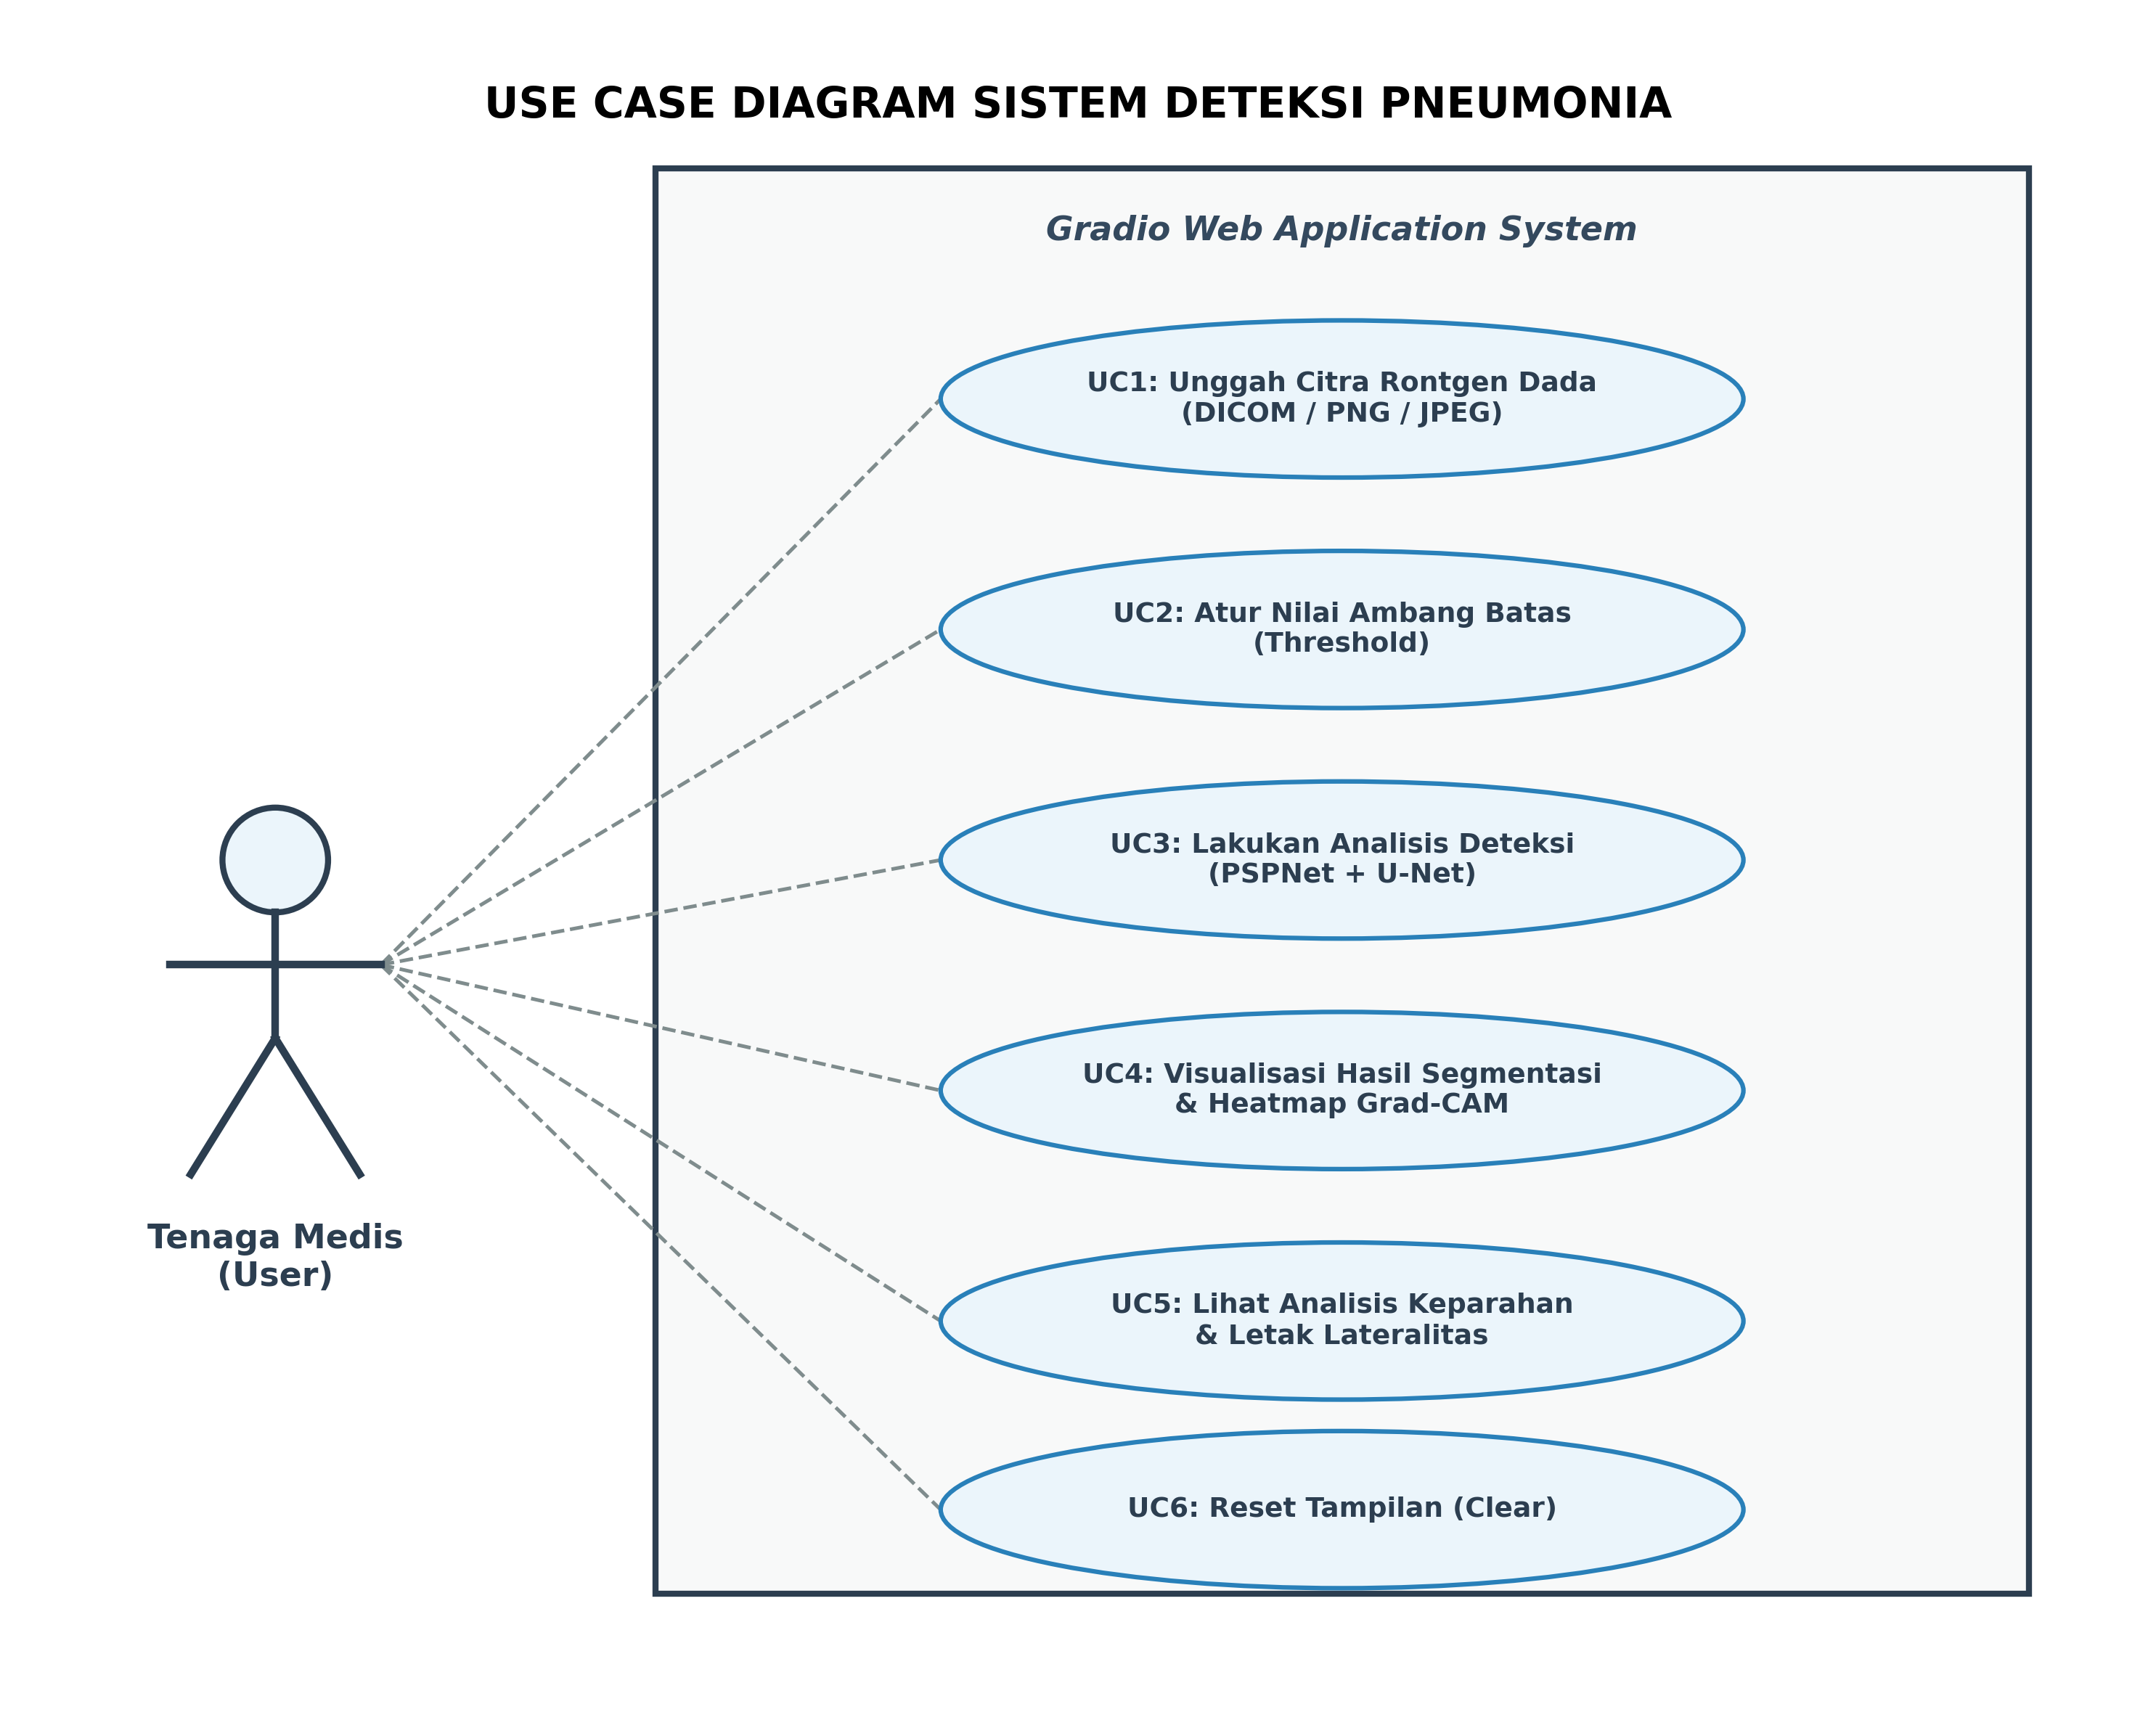
\includegraphics[width=\linewidth]{gambar/ip_address_vps.png}
\caption{IP Address VPS}
\label{fig:ip_address_vps}
\end{figure}

Lingkungan server menggunakan sistem operasi Linux yang dikonfigurasi dengan menyesuaikan kebutuhan \textit{runtime} aplikasi, termasuk Spring Boot untuk \textit{backend} dan SolidJS untuk \textit{frontend}. Seluruh layanan pendukung seperti PostgreSQL dan Redis dijalankan dalam lingkungan Docker yang memudahkan pengelolaan kontainer, replikasi layanan, serta \textit{deployment} yang konsisten.

% ============================================================================
% PENUTUP
% ============================================================================
\section{Penutup}

\subsection{Kesimpulan}

Berdasarkan hasil analisis, perancangan, implementasi, serta uji coba yang telah dilakukan terhadap sistem \textit{e-commerce} multi-seller NiagaNow, dapat disimpulkan bahwa sistem ini berhasil dibangun dengan memenuhi kebutuhan utama dari sebuah platform marketplace modern. Sistem telah mencakup fitur-fitur penting seperti manajemen toko, pengelolaan katalog produk, proses pemesanan dan \textit{checkout} oleh pembeli, serta integrasi pembayaran dengan Xendit melalui pemrosesan \textit{event webhook} secara \textit{real-time}. Seluruh fitur tersebut berfungsi sesuai dengan ekspektasi dan telah melalui serangkaian pengujian fungsional yang valid.

Secara teknologi, penggunaan Spring Boot sebagai kerangka kerja \textit{backend} dan SolidJS di sisi \textit{frontend} terbukti efektif dalam menghasilkan aplikasi yang responsif, modular, serta mudah dikembangkan. Penggunaan PostgreSQL sebagai sistem basis data turut mendukung konsistensi dan efisiensi penyimpanan data, terutama dalam menangani transaksi dan aktivitas pengguna. Dari sisi antarmuka, desain halaman-halaman utama seperti \textit{Store Dashboard}, \textit{Order Details}, dan \textit{Add Products} dirancang dengan prinsip modularitas dan responsivitas, sehingga memberikan pengalaman pengguna yang intuitif dan informatif.

Keandalan sistem juga terlihat dari hasil simulasi \textit{webhook} yang menunjukkan bahwa sistem dapat memperbarui status transaksi secara tepat waktu dan akurat. Secara keseluruhan, sistem telah menunjukkan performa yang baik dalam aspek teknis maupun fungsional, serta dinyatakan siap untuk digunakan secara operasional. Prototipe sistem dapat diakses melalui laman \url{https://niaganow.site} sebagai implementasi nyata dari hasil penelitian ini.

\subsection{Saran}

Sebagai tindak lanjut dari implementasi sistem NiagaNow, terdapat beberapa saran pengembangan yang dapat dijadikan acuan untuk peningkatan ke depan:
\begin{enumerate}
    \item Optimasi lebih lanjut untuk mendukung skalabilitas sistem, terutama dalam menghadapi lonjakan jumlah pengguna dan transaksi yang besar.
    \item Peningkatan fitur keamanan seperti autentikasi dua faktor (2FA) dan enkripsi \textit{end-to-end} untuk memperkuat perlindungan data sensitif pengguna.
    \item Integrasi teknologi kecerdasan buatan (AI) untuk meningkatkan personalisasi pengalaman pengguna, misalnya melalui rekomendasi produk yang disesuaikan dengan preferensi atau riwayat pembelian.
    \item Penambahan fitur laporan penjualan bagi penjual agar dapat memantau performa produk melalui metrik seperti tingkat konversi dan demografi pembeli.
    \item Pengembangan aplikasi \textit{mobile} agar platform lebih mudah diakses dari berbagai perangkat.
    \item Penyediaan panduan atau tutorial interaktif untuk membantu proses \textit{onboarding} pengguna baru, khususnya penjual.
    \item Pelaksanaan \textit{monitoring} dan \textit{maintenance} sistem secara berkala guna memastikan kestabilan dan keamanan jangka panjang.
\end{enumerate}

% ============================================================================
% DAFTAR PUSTAKA
% ============================================================================
% Option 1: Using BibTeX (recommended)
% \bibliography{referensi}

% Option 2: Manual bibliography (inline)
\begin{thebibliography}{99}

\bibitem[Amelia \& Bernard(2023)]{amelia2023}
Amelia, D.~R., \& Bernard, J.
\newblock 2023.
\newblock ``Pengaruh E-Service Quality dan Kepercayaan Kepuasan Pelanggan pada Marketplace Tokopedia.''
\newblock \emph{Jurnal Riset Manajemen Dan Ekonomi (RIME)}, 1(4), 519--527.

\bibitem[Astuti \& Fathoni(2019)]{astuti2019}
Astuti, Y., \& Fathoni, A.
\newblock 2019.
\newblock ``Peran E-Commerce Peningkatan Pendapatan Usaha Mikro Kecil dan Menengah di Kota Semarang.''
\newblock \emph{Jurnal Riset Ekonomi Dan Bisnis}, 12(1), 1--9.

\bibitem[Aziz \& Destyningtias(2022)]{aziz2022}
Aziz, F., \& Destyningtias, Y.
\newblock 2022.
\newblock ``Implementasi TypeScript pada Pengembangan Aplikasi Web Frontend untuk Peningkatan Kualitas Kode.''
\newblock \emph{Jurnal Teknologi Informasi dan Ilmu Komputer (JTIIK)}, 9(4), 725--732.

\bibitem[Fahlevi \& Setiadi(2021)]{fahlevi2021}
Fahlevi, M.~R., \& Setiadi, D.
\newblock 2021.
\newblock ``Implementasi Teknologi Kontainer Docker untuk Deployment Aplikasi Web pada Server.''
\newblock \emph{Jurnal Sistem dan Teknologi Informasi (JUSTIN)}, 9(3), 294--299.

\bibitem[Hendri dkk.(2020)]{hendri2020}
Hendri, J.~W.~H.~M., Ferian, R.~A., Faharrudin, W., \& Hanaatmoko, Y.~Y.
\newblock 2020.
\newblock ``Pengujian Black Box pada Aplikasi Sistem Informasi Pengelolaan Masjid Menggunakan Teknik Equivalence Partitions.''
\newblock \emph{Jurnal Teknologi Sistem Informasi dan Aplikasi}, ISSN 2654-3788.

\bibitem[Hidayat(2020)]{hidayat2020}
Hidayat, A.
\newblock 2020.
\newblock ``Rancang Bangun Aplikasi Marketplace untuk Produk Pertanian Berbasis Web.''
\newblock \emph{Jurnal Teknologi Dan Sistem Informasi (JTSI)}, 1(2), 76--83.

\bibitem[Kadir(2018)]{kadir2018}
Kadir, A.
\newblock 2018.
\newblock \emph{Dasar-Dasar Jaringan Komputer dan Web}.
\newblock Andi Publisher.

\bibitem[Munawar(2021)]{munawar2021}
Munawar, Z.
\newblock 2021.
\newblock ``Model Bisnis E-Commerce di Indonesia: Studi Kasus pada Perusahaan Startup.''
\newblock \emph{Jurnal Informatika: Jurnal Pengembangan IT}, 6(2), 67--73.

\bibitem[Noerdiansyah dkk.(2024)]{noerdiansyah2024}
Noerdiansyah, S., Rifaldi, M., Lathif, F., \& Putra, R.
\newblock 2024.
\newblock ``Analisa Dan Perancangan Sistem E-Commerce Sepatu Dengan Menggunakan UML (Studi Kasus: Kickstyle).''
\newblock \emph{Jurnal Ilmu Komputer}, 7(1), 72--79.

\bibitem[Nurcholis \& Sipan(2021)]{nurcholis2021}
Nurcholis, A., \& Sipan, M.
\newblock 2021.
\newblock ``Analisis Pengalaman Pelanggan pada E-commerce C2C di Indonesia.''
\newblock \emph{Jurnal Sains Pemasaran Indonesia}, 20(2), 115--130.

\bibitem[Pranata \& Sukamto(2023)]{pranata2023}
Pranata, A.~D., \& Sukamto, R.~A.
\newblock 2023.
\newblock ``Pengembangan Aplikasi Backend Menggunakan Framework Spring Boot untuk Sistem Manajemen Inventori.''
\newblock \emph{Jurnal Pengembangan Teknologi Informasi dan Ilmu Komputer}, 7(2), 845--853.

\bibitem[Prastyaningtyas \& Haryono(2020)]{prastyaningtyas2020}
Prastyaningtyas, E.~W., \& Haryono, A.~T.
\newblock 2020.
\newblock ``Pengaruh Kualitas Produk, Harga dan Kualitas Pelayanan Keputusan Pembelian pada E-commerce Traveloka.''
\newblock \emph{Diponegoro Journal of Management}, 9(3).

\bibitem[Purbo(2015)]{purbo2015}
Purbo, O.~W.
\newblock 2015.
\newblock \emph{Buku Pegangan untuk Sekolah dan UKM: Membangun Server dengan Debian 8 Jessie}.
\newblock Elex Media Komputindo.

\bibitem[Putra \& Mulyani(2022)]{putra2022}
Putra, A.~N., \& Mulyani, A.
\newblock 2022.
\newblock ``Analisis Komparatif Kinerja Editor Kode Visual Studio Code dan Sublime Text dalam Pengembangan Proyek Web.''
\newblock \emph{Jurnal Informatika Universitas Pamulang}, 7(1), 112--119.

\bibitem[Raharjo(2018)]{raharjo2018}
Raharjo, B.
\newblock 2018.
\newblock \emph{Belajar Otodidak Membuat RESTful Web Service dengan Framework CodeIgniter}.
\newblock Informatika.

\bibitem[Saputra \& Afrianto(2020)]{saputra2020}
Saputra, D.~D., \& Afrianto, I.
\newblock 2020.
\newblock ``Implementasi Redis sebagai Cache untuk Mengoptimalkan Kinerja Query Database pada Aplikasi E-Commerce.''
\newblock \emph{Jurnal Teknika}, 12(1), 45--52.

\bibitem[Setiadi dkk.(2023)]{setiadi2023}
Setiadi, T., Fajri, L.~R.~H.~A., \& Ilhami, S.~D.
\newblock 2023.
\newblock ``Penerapan Sistem Informasi Untuk Survei Marketplace dalam Bisnis Kreatif UMKM Berbasis E-commerce.''
\newblock \emph{Jurnal Ilmiah Sistem Informasi}, 2(2), 16--29.

\bibitem[Siddiq(2018)]{siddiq2018}
Siddiq, M.
\newblock 2018.
\newblock \emph{Pemrograman Web dengan HTML, CSS, dan JavaScript}.
\newblock CV. Lokomedia.

\bibitem[Simarmata dkk.(2022)]{simarmata2022}
Simarmata, J., dkk.
\newblock 2022.
\newblock \emph{E-Commerce: Implementasi, Strategi dan Inovasinya}.
\newblock Yayasan Kita Menulis.

\bibitem[Siregar \& Khair(2022)]{siregar2022}
Siregar, S.~A., \& Khair, H.
\newblock 2022.
\newblock ``Implementasi JSON Web Token (JWT) untuk Sistem Otentikasi dan Otorisasi pada Aplikasi Web Berbasis REST API.''
\newblock \emph{Jurnal Sains Komputer \& Informatika (J-SAKTI)}, 6(1), 449--460.

\bibitem[Sukamto \& Shalahuddin(2018)]{sukamto2018}
Sukamto, R.~A., \& Shalahuddin, M.
\newblock 2018.
\newblock \emph{Rekayasa Perangkat Lunak (Terstruktur dan Berorientasi Objek)}.
\newblock Informatika.

\bibitem[Yasin(2022)]{yasin2022}
Yasin, M.
\newblock 2022.
\newblock ``Pemanfaatan Framework Utility-First Tailwind CSS untuk Mempercepat Pengembangan Antarmuka Website Responsif.''
\newblock \emph{Jurnal Buana Informatika}, 13(1), 35--44.

\bibitem[Yuliana(2004)]{yuliana2004}
Yuliana, O.
\newblock 2004.
\newblock ``Penggunaan Teknologi Internet dalam Bisnis.''
\newblock \emph{Jurnal Akuntansi Dan Keuangan}, 2(1), 36--52.
\newblock \url{https://doi.org/10.9744/jak.2.1.pp.36-52}.

\end{thebibliography}

\end{document}
